\chapter{Modeling running time}\label{chapmodelruntime}

\begin{objectives} \label[objectives]{Formally-modeling-running}

\begin{itemize}
\tightlist
\item
  Formally modeling running time, and in particular notions such as
  \(O(n)\) or \(O(n^3)\) time algorithms.\\
\item
  The classes \(\mathbf{P}\) and \(\mathbf{EXP}\) modelling polynomial
  and exponential time respectively.\\
\item
  The \emph{time hierarchy theorem}, that in particular says that for
  every \(k \geq 1\) there are functions we \emph{can} compute in
  \(O(n^{k+1})\) time but \emph{can not} compute in \(O(n^k)\) time.
\item
  The class \(\mathbf{P_{/poly}}\) of \emph{non uniform} computation and
  the result that \(\mathbf{P} \subseteq \mathbf{P_{/poly}}\)
\end{itemize}

\end{objectives}

\begin{quote}
``When the measure of the problem-size is reasonable and when the sizes
assume values arbitrarily large, an asymptotic estimate of \ldots{} the
order of difficulty of {[}an{]} algorithm .. is theoretically important.
It cannot be rigged by making the algorithm artificially difficult for
smaller sizes'', Jack Edmonds, ``Paths, Trees, and Flowers'', 1963
\end{quote}

\begin{quote} \label[quote]{Max-Newman-It-is-all-very}

\emph{Max Newman:} It is all very well to say that a machine could
\ldots{} do this or that, but \ldots{} what about the time it would take
to do it?

\emph{Alan Turing:} To my mind this time factor is the one question
which will involve all the real technical difficulty.

BBC radio panel on ``Can automatic Calculating Machines Be Said to
Think?'', 1952

\end{quote}

In \cref{chapefficient} we saw examples of efficient algorithms, and
made some claims about their running time, but did not give a
mathematically precise definition for this concept. We do so in this
chapter, using the models of Turing machines and RAM machines (or
equivalently NAND-TM and NAND-RAM) we have seen before. The running time
of an algorithm is not a fixed number since any non-trivial algorithm
will take longer to run on longer inputs. Thus, what we want to measure
is the \emph{dependence} between the number of steps the algorithms
takes and the length of the input. In particular we care about the
distinction between algorithms that take at most \emph{polynomial time}
(i.e., \(O(n^c)\) time for some constant \(c\)) and problems for which
every algorithm requires at least \emph{exponential time} (i.e.,
\(\Omega(2^{n^c})\) for some \(c\)). As mentioned in Edmond's quote in
\cref{chapefficient}, the difference between these two can sometimes be
as important as the difference between being computable and
uncomputable.


\begin{figure}
\centering
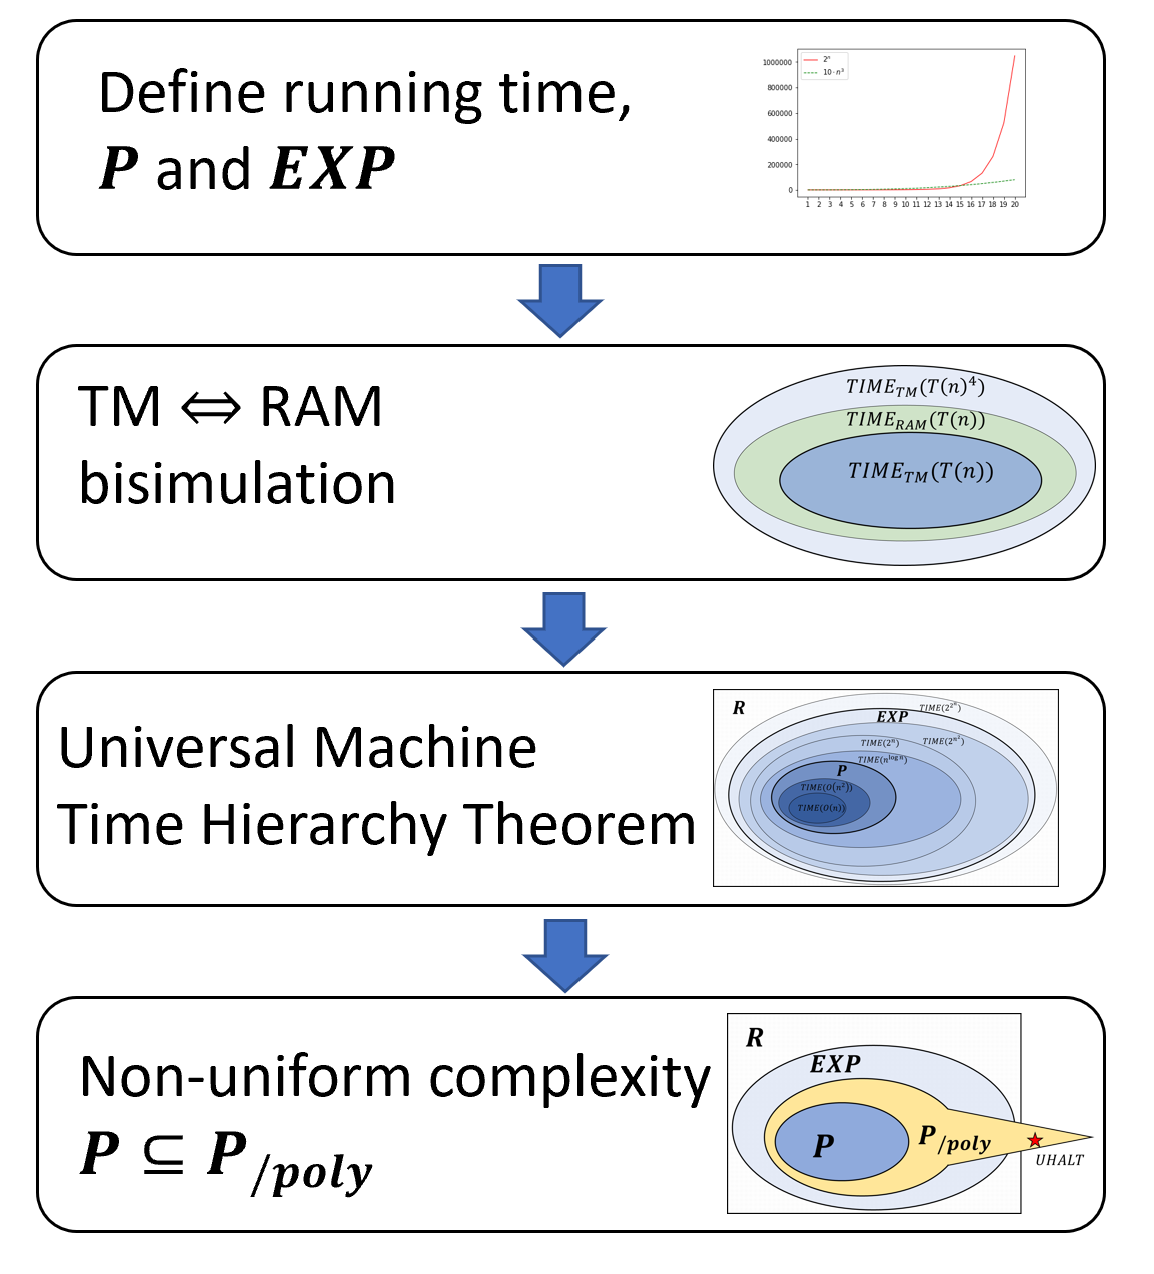
\includegraphics[width=\textwidth, height=0.25\paperheight, keepaspectratio]{../figure/runtimeoverview.png}
\caption{Overview of the results of this chapter.}
\label{runtimeoverviewfig}
\end{figure}

In this chapter we formally define the notion of a function being
computable in \(T(n)\) time where \(T\) is some function mapping the
length of the input to a bound on the number of computation steps. We
then do the following (see also \cref{runtimeoverviewfig}):

\begin{itemize}
\item
  Define the class \(\mathbf{P}\) of Boolean functions that can be
  computed in polynomial time and its superset \(\mathbf{EXP}\) of
  functions that can be computed in exponential time.
\item
  Show that the time to compute a function using a Turing Machine and
  using a RAM machine (or NAND-RAM program) is \emph{polynomially
  related} which in particular means that the classes \(\mathbf{P}\) and
  \(\mathbf{EXP}\) can be equivalently defined using either Turing
  Machines or RAM machines / NAND-RAM programs.
\item
  Give an \emph{efficient} universal NAND-RAM program and use this to
  establish the \emph{time hierarchy theorem} that in particular implies
  that \(\mathbf{P} \subsetneq \mathbf{EXP}\).
\item
  We relate the notions defined here to the \emph{non uniform} models of
  Boolean circuits and NAND-CIRC programs defined in \cref{compchap}. We
  define \(\mathbf{P_{/poly}}\) to be the class of functions computed by
  a \emph{sequence} of polynomial-sized circuits. We prove that
  \(\mathbf{P} \subseteq \mathbf{P_{/poly}}\) and that
  \(\mathbf{P_{/poly}}\) contains \emph{uncomputable} functions.
\end{itemize}

\section{Formally defining running
time}\label{Formally-defining-running}

Our models of computation such Turing Machines, NAND-TM and NAND-RAM
programs and others all operate by executing a sequence of instructions
on an input one step at a time. We can define the \emph{running time} of
an algorithm \(M\) in one of these models by measuring the number of
steps \(M\) takes on input \(x\) as a \emph{function of the length
\(|x|\) of the input}. We start by defining running time with respect to
Turing Machines:

\hypertarget{time-TM-def}{}
\begin{definition}[Running time (Turing Machines)] \label[definition]{time-TM-def}

Let \(T:\N \rightarrow \N\) be some function mapping natural numbers to
natural numbers. We say that a function
\(F:\{0,1\}^* \rightarrow \{0,1\}^*\) is \emph{computable in \(T(n)\)
Single-Tape-Turing-Machine time (TM-time for short)} if there exists a
Turing Machine \(M\) such that for every sufficiently large \(n\) and
every \(x\in \{0,1\}^n\), when given input \(x\), the machine \(M\)
halts after executing at most \(T(n)\) steps and outputs \(F(x)\).

We define \(\ensuremath{\mathit{TIME}}_{\mathsf{TM}}(T(n))\) to be the
set of Boolean functions (functions mapping \(\{0,1\}^*\) to
\(\{0,1\}\)) that are computable in \(T(n)\) TM time.

\end{definition}

\hypertarget{formaldefinetime}{}
\begin{bigidea} \label[bigidea]{formaldefinetime}

For a function \(F:\{0,1\}^* \rightarrow \{0,1\}\) and
\(T:\N \rightarrow \N\), we can formally define what it means for \(F\)
to be computable in time at most \(T(n)\) where \(n\) is the size of the
input.

\end{bigidea}

\begin{pause} \label[pause]{creftime-TM-def-is-not-ve}

\cref{time-TM-def} is not very complicated but is one of the most
important definitions of this book. As usual,
\(\ensuremath{\mathit{TIME}}_{\mathsf{TM}}(T(n))\) is a class of
\emph{functions}, not of \emph{machines}. If \(M\) is a Turing Machine
then a statement such as ``\(M\) is a member of
\(\ensuremath{\mathit{TIME}}_{\mathsf{TM}}(n^2)\)'' does not make sense.

\end{pause}

The relaxation of considering only ``sufficiently large'' \(n\)'s is not
very important but it is convenient since it allows us to avoid dealing
explicitly with un-interesting ``edge cases''. In most cases we will
anyway be interested in determining running time only up to constant and
even polynomial factors. Note that we can always compute a function on a
finite number of inputs using a lookup table.

While the notion of being computable within a certain running time can
be defined for every function, the class
\(\ensuremath{\mathit{TIME}}_{\mathsf{TM}}(T(n))\) is a class of
\emph{Boolean functions} that have a single bit of output. This choice
is not very important, but is made for simplicity and convenience later
on. In fact, every non-Boolean function has a computationally equivalent
Boolean variant, see \cref{boolex}.

\hypertarget{timeboundexample}{}
\begin{solvedexercise}[Example of time bounds] \label[solvedexercise]{timeboundexample}

Prove that
\(\ensuremath{\mathit{TIME}}_{\mathsf{TM}}(10\cdot n^3) \subseteq \ensuremath{\mathit{TIME}}_{\mathsf{TM}}(2^n)\).

\end{solvedexercise}


\begin{marginfigure}
\centering
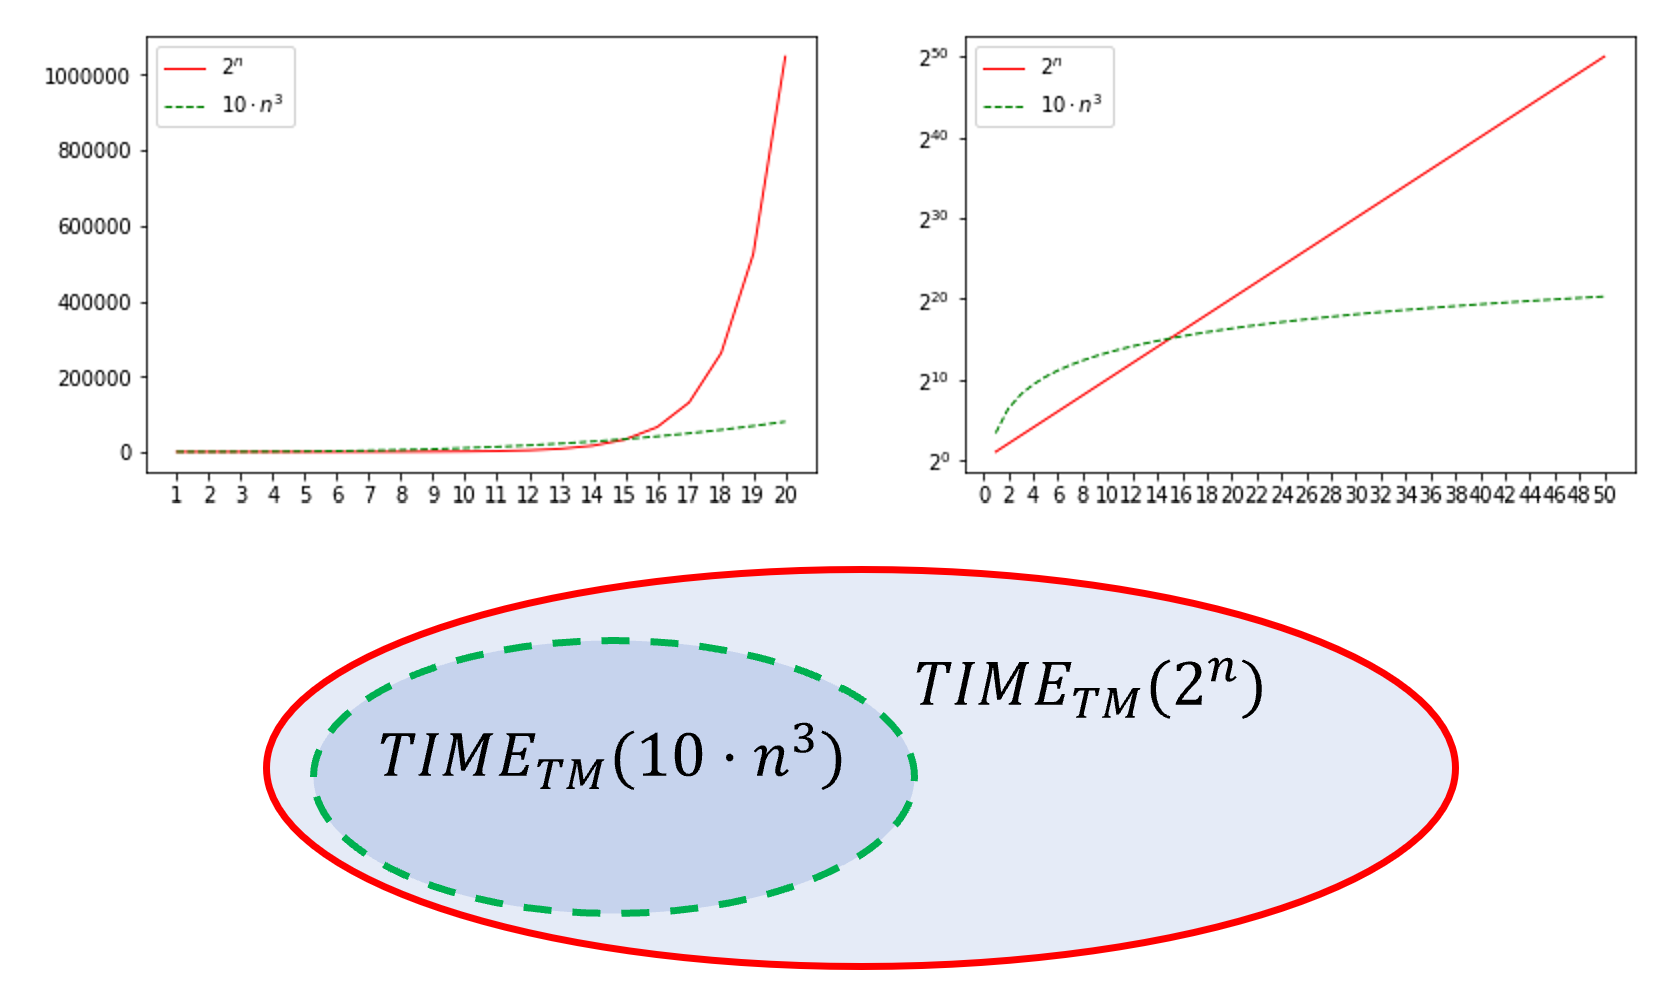
\includegraphics[width=\linewidth, height=1.5in, keepaspectratio]{../figure/exampletimebounds.png}
\caption{Comparing \(T(n)=10n^3\) with \(T'(n) = 2^n\) (on the right
figure the Y axis is in log scale). Since for every large enough \(n\),
\(T'(n) \geq T(n)\),
\(\ensuremath{\mathit{TIME}}_{\mathsf{TM}}(T(n)) \subseteq \ensuremath{\mathit{TIME}}_{\mathsf{TM}}(T'(n))\).}
\label{examplefimeboundsfig}
\end{marginfigure}

\begin{solution} \label[solution]{The-proof-is-illustrated-}

The proof is illustrated in \cref{examplefimeboundsfig}. Suppose that
\(F\in \ensuremath{\mathit{TIME}}_{\mathsf{TM}}(10\cdot n^3)\) and hence
there some number \(N_0\) and a machine \(M\) such that for every
\(n> N_0\), and \(x\in \{0,1\}^*\), \(M(x)\) outputs \(F(x)\) within at
most \(10\cdot n^3\) steps. Since \(10\cdot n^3 = o(2^n)\), there is
some number \(N_1\) such that for every \(n>N_1\),
\(10\cdot n^3 < 2^n\). Hence for every \(n > \max\{ N_0, N_1 \}\),
\(M(x)\) will output \(F(x)\) within at most \(2^n\) steps, just
demonstrating that
\(F \in \ensuremath{\mathit{TIME}}_{\mathsf{TM}}(2^n)\).

\end{solution}

\subsection{Polynomial and Exponential
Time}\label{Polynomial-and-Exponentia}

Unlike the notion of computability, the exact running time can be a
function of the model we use. However, it turns out that if we only care
about ``coarse enough'' resolution (as will most often be the case) then
the choice of the model, whether Turing Machines, RAM machines,
NAND-TM/NAND-RAM programs, or C/Python programs, does not matter. This
is known as the \emph{extended} Church-Turing Thesis. Specifically we
will mostly care about the difference between \emph{polynomial} and
\emph{exponential} time.

The two main time complexity classes we will be interested in are the
following:

\begin{itemize}
\item
  \textbf{Polynomial time:} A function
  \(F:\{0,1\}^* \rightarrow \{0,1\}\) is \emph{computable in polynomial
  time} if it is in the class
  \(\mathbf{P} = \cup_{c\in \{1,2,3,\ldots \}} \ensuremath{\mathit{TIME}}_{\mathsf{TM}}(n^c)\).
  That is, \(F\in \mathbf{P}\) if there is an algorithm to compute \(F\)
  that runs in time at most \emph{polynomial} (i.e., at most \(n^c\) for
  some constant \(c\)) in the length of the input.
\item
  \textbf{Exponential time:} A function
  \(F:\{0,1\}^* \rightarrow \{0,1\}\) is \emph{computable in exponential
  time} if it is in the class
  \(\mathbf{EXP} = \cup_{c\in \{1,2,3,\ldots \}} \ensuremath{\mathit{TIME}}_{\mathsf{TM}}(2^{n^c})\).
  That is, \(F\in \mathbf{EXP}\) if there is an algorithm to compute
  \(F\) that runs in time at most \emph{exponential} (i.e., at most
  \(2^{n^c}\) for some constant \(c\)) in the length of the input.
\end{itemize}

In other words, these are defined as follows:

\hypertarget{PandEXPdef}{}
\begin{definition}[$\mathbf{P}$ and $\mathbf{EXP}$] \label[definition]{PandEXPdef}

Let \(F:\{0,1\}^* \rightarrow \{0,1\}\). We say that \(F\in \mathbf{P}\)
if there is a polynomial \(p:\N \rightarrow \R\) and a Turing Machine
\(M\) such that for every \(x\in \{0,1\}^*\), when given input \(x\),
the Turing machine halts within at most \(p(|x|)\) steps and outputs
\(F(x)\).

We say that \(F\in \mathbf{EXP}\) if there is a polynomial
\(p:\N \rightarrow \R\) and a Turing Machine \(M\) such that for every
\(x\in \{0,1\}^*\), when given input \(x\), \(M\) halts within at most
\(2^{p(|x|)}\) steps and outputs \(F(x)\).

\end{definition}

\begin{pause} \label[pause]{Please-take-the-time-to-m}

Please take the time to make sure you understand these definitions. In
particular, sometimes students think of the class \(\mathbf{EXP}\) as
corresponding to functions that are \emph{not} in \(\mathbf{P}\).
However, this is not the case. If \(F\) is in \(\mathbf{EXP}\) then it
\emph{can} be computed in exponential time. This does not mean that it
cannot be computed in polynomial time as well.

\end{pause}

\hypertarget{diffdefofP}{}
\begin{solvedexercise}[Differerent definitions of $\mathbf{P}$] \label[solvedexercise]{diffdefofP}

Prove that \(\mathbf{P}\) as defined in \cref{PandEXPdef} is equal to
\(\cup_{c\in \{1,2,3,\ldots \}} \ensuremath{\mathit{TIME}}_{\mathsf{TM}}(n^c)\)

\end{solvedexercise}

\begin{solution} \label[solution]{To-show-these-two-sets-ar}

To show these two sets are equal we need to show that
\(\mathbf{P} \subseteq \cup_{c\in \{1,2,3,\ldots \}} \ensuremath{\mathit{TIME}}_{\mathsf{TM}}(n^c)\)
and
\(\cup_{c\in \{1,2,3,\ldots \}} \ensuremath{\mathit{TIME}}_{\mathsf{TM}}(n^c) \subseteq \mathbf{P}\).
We start with the former inclusion. Suppose that \(F \in \mathbf{P}\).
Then there is some polynomial \(p:\N \rightarrow \R\) and a Turing
machine \(M\) such that \(M\) computes \(F\) and \(M\) halts on every
input \(x\) within at most \(p(|x|)\) steps. We can write the polynomial
\(p:\N \rightarrow \R\) in the form \(p(n) = \sum_{i=0}^d a_i n^i\)
where \(a_0,\ldots,a_d \in \R\), and we assume that \(a_d\) is nonzero
(or otherwise we just let \(d\) correspond to the largest number such
that \(a_d\) is nonzero). The \emph{degree} if \(p\) the number \(d\).
Since \(n^d = o(n^{d+1})\), no matter what is the coefficient \(a_d\),
for large enough \(n\), \(p(n) < n^{d+1}\) which means that the Turing
machine \(M\) will halt on inputs of length \(n\) within fewer than
\(n^{d+1}\) steps, and hence
\(F \in \ensuremath{\mathit{TIME}}_{\mathsf{TM}}(n^{d+1}) \subseteq \cup_{c\in \{1,2,3,\ldots \}} \ensuremath{\mathit{TIME}}_{\mathsf{TM}}(n^c)\).

For the second inclusion, suppose that
\(F \in \cup_{c\in \{1,2,3,\ldots \}} \ensuremath{\mathit{TIME}}_{\mathsf{TM}}(n^c)\).
Then there is some positive \(c \in \N\) such that
\(F \in \ensuremath{\mathit{TIME}}_{\mathsf{TM}}(n^c)\) which means that
there is a Turing Machine \(M\) and some number \(N_0\) such that \(M\)
computes \(F\) and for every \(n>N_0\), \(M\) halts on length \(n\)
inputs within at most \(n^c\) steps. Let \(T_0\) be the maximum number
of steps that \(M\) takes on inputs of length at most \(N_0\). Then if
we define the polynomial \(p(n) = n^c + T_0\) then we see that \(M\)
halts on every input \(x\) within at most \(p(|x|)\) steps and hence the
existence of \(M\) demonstrates that \(F\in \mathbf{P}\).

\end{solution}

Since exponential time is much larger than polynomial time,
\(\mathbf{P}\subseteq \mathbf{EXP}\). All of the problems we listed in
\cref{chapefficient} are in \(\mathbf{EXP}\), but as we've seen, for
some of them there are much better algorithms that demonstrate that they
are in fact in the smaller class \(\mathbf{P}\).

\begin{longtable}[]{@{}ll@{}}
\toprule
\(\mathbf{P}\) & \(\mathbf{EXP}\) (but not known to be in
\(\mathbf{P}\))\tabularnewline
\midrule
\endhead
Shortest path & Longest Path\tabularnewline
Min cut & Max cut\tabularnewline
2SAT & 3SAT\tabularnewline
Linear eqs & Quad. eqs\tabularnewline
Zerosum & Nash\tabularnewline
Determinant & Permanent\tabularnewline
Primality & Factoring\tabularnewline
\bottomrule
\end{longtable}

Table : A table of the examples from \cref{chapefficient}. All these
problems are in \(\mathbf{EXP}\) but the only the ones on the left
column are currently known to be in \(\mathbf{P}\) as well (i.e., they
have a polynomial-time algorithm). See also \cref{PvsEXPfig}.


\begin{marginfigure}
\centering
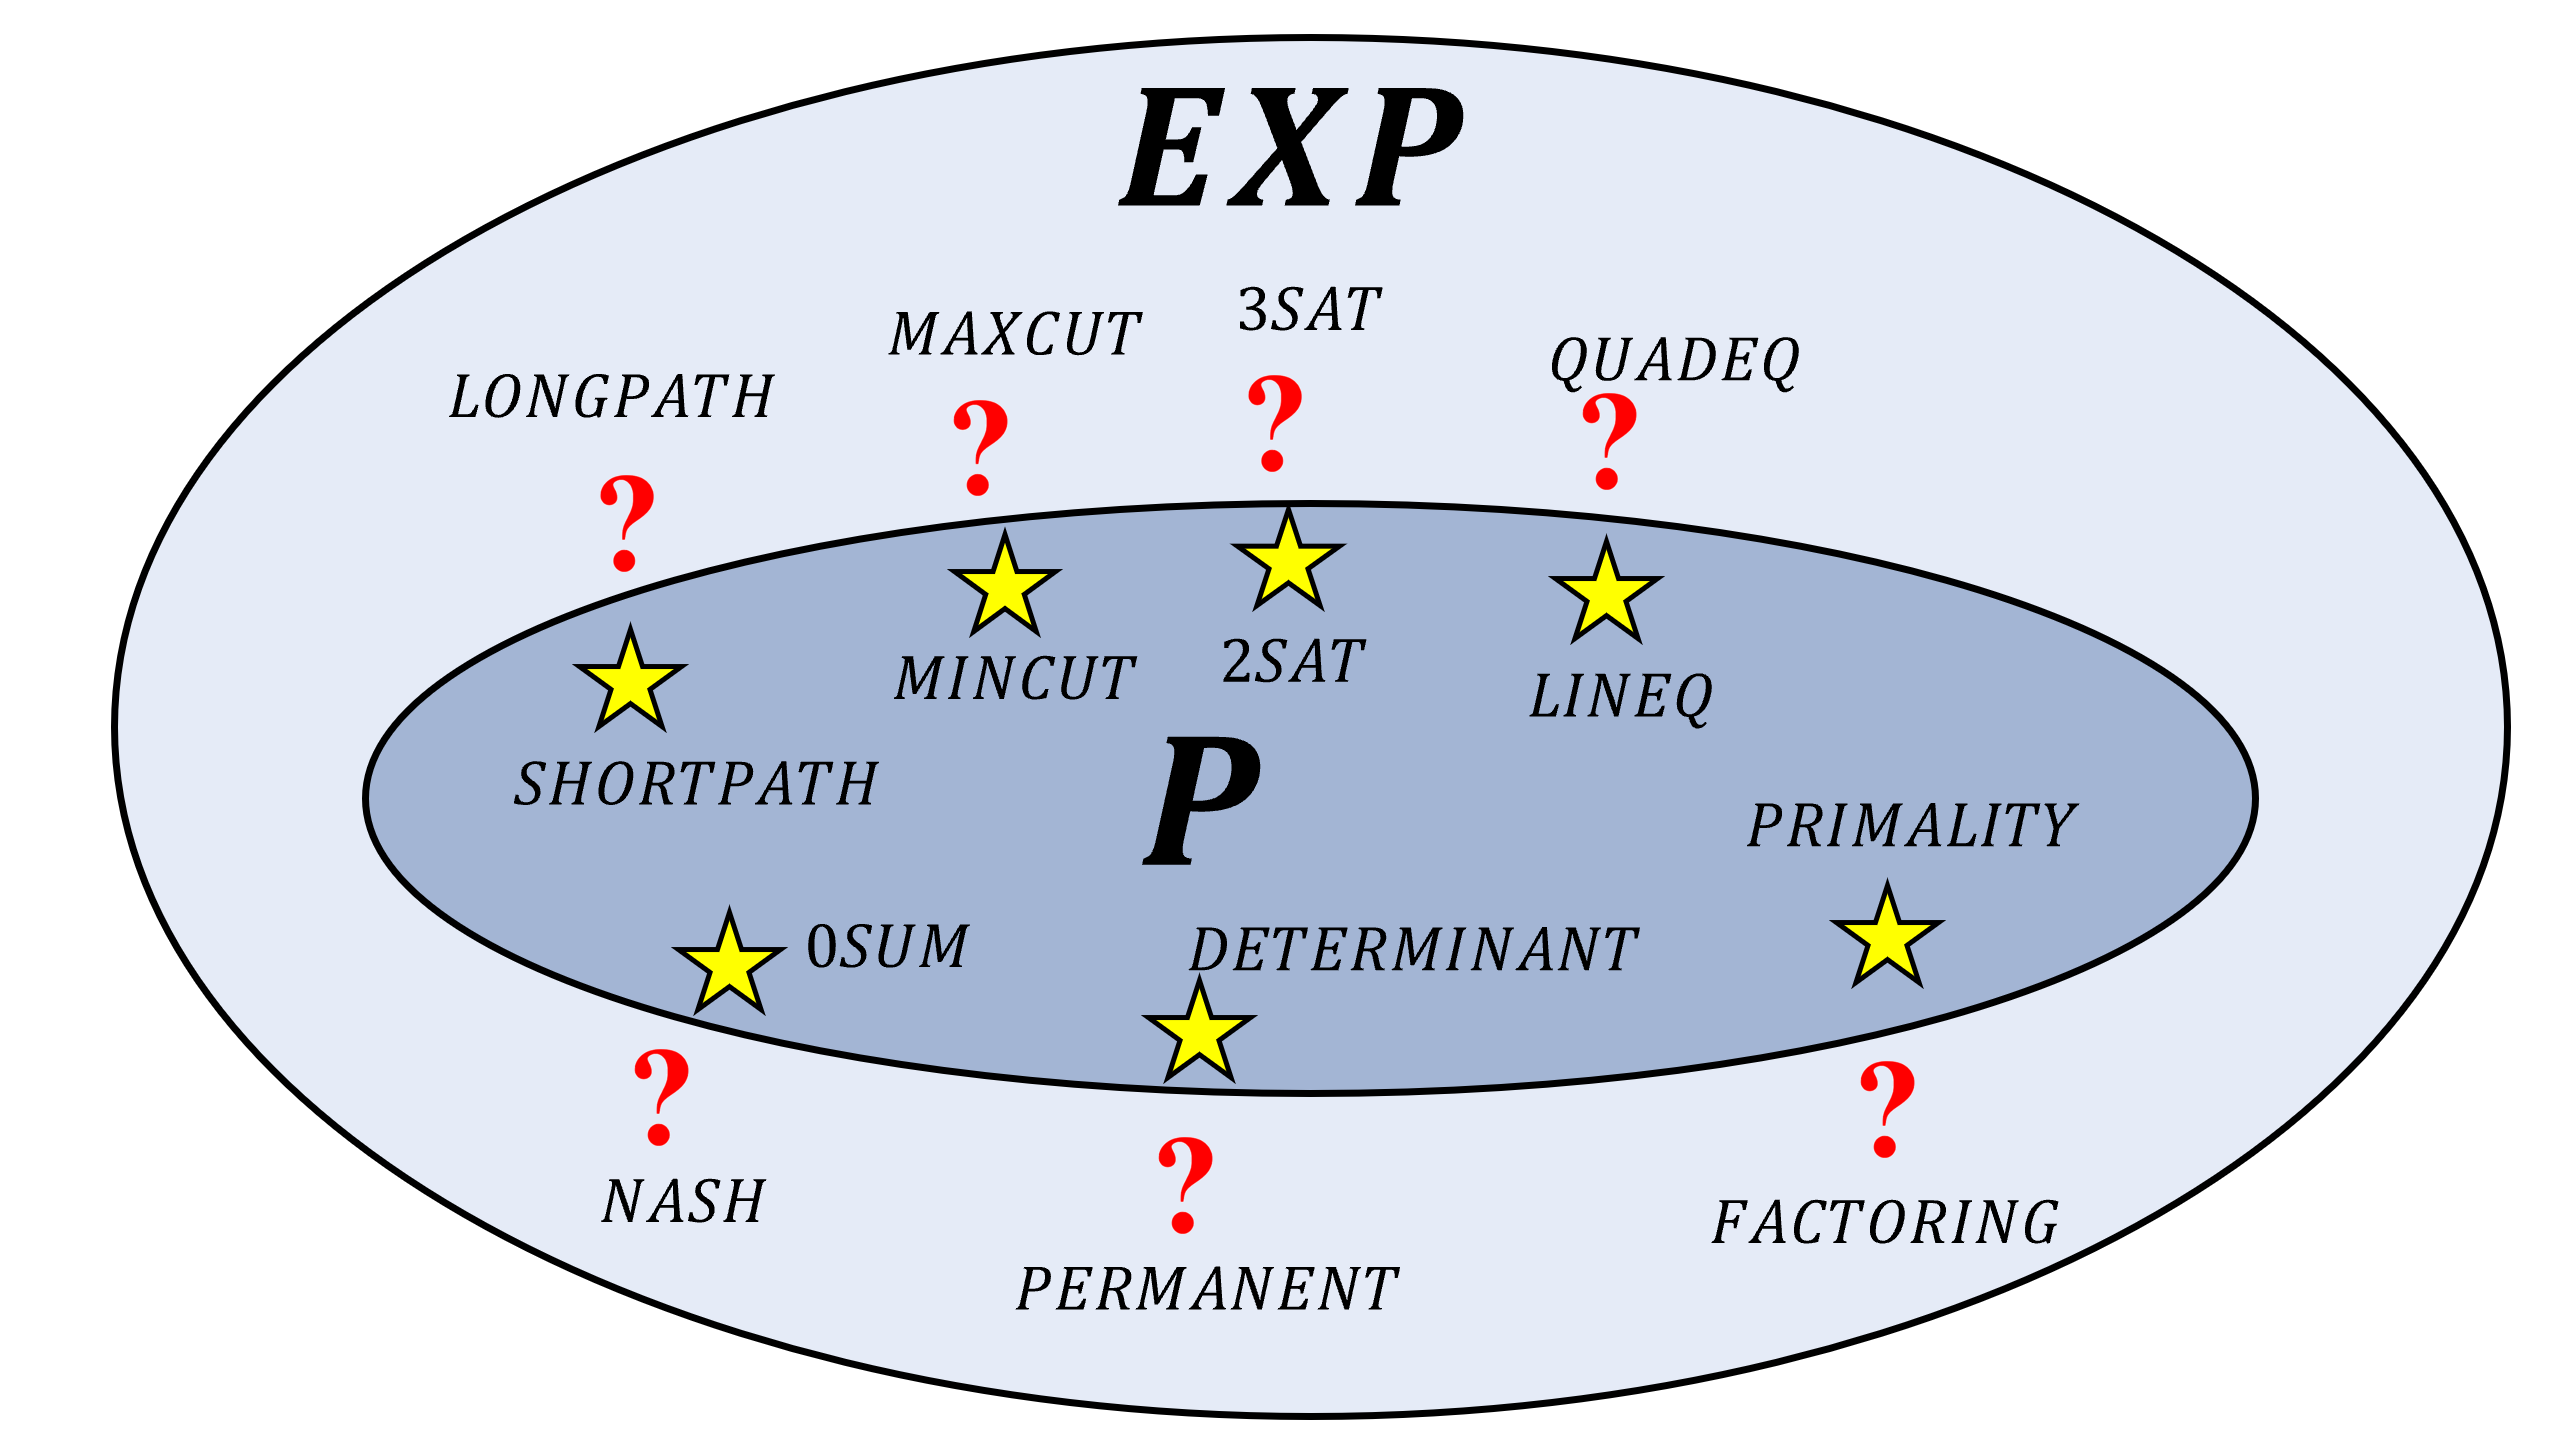
\includegraphics[width=\linewidth, height=1.5in, keepaspectratio]{../figure/PvsEXP.png}
\caption{Some examples of problems that are known to be in
\(\mathbf{P}\) and problems that are known to be in \(\mathbf{EXP}\) but
not known whether or not they are in \(\mathbf{P}\). Since both
\(\mathbf{P}\) and \(\mathbf{EXP}\) are classes of Boolean functions, in
this figure we always refer to the \emph{Boolean} (i.e., Yes/No) variant
of the problems.}
\label{PvsEXPfig}
\end{marginfigure}

\hypertarget{booleanversion}{}
\begin{remark}[Boolean versions of problems] \label[remark]{booleanversion}

Many of the problems defined in \cref{chapefficient} correspond to
\emph{non Boolean} functions (functions with more than one bit of
output) while \(\mathbf{P}\) and \(\mathbf{EXP}\) are sets of Boolean
functions. However, for every non-Boolean function \(F\) we can always
define a computationally-equivalent Boolean function \(G\) by letting
\(G(x,i)\) be the \(i\)-th bit of \(F(x)\) (see \cref{boolex}). Hence
the table above, as well as \cref{PvsEXPfig}, refer to the
computationally-equivalent Boolean variants of these problems.

\end{remark}

\section{Modeling running time using RAM Machines /
NAND-RAM}\label{Modeling-running-time-usi}

Turing Machines are a clean theoretical model of computation, but do not
closely correspond to real-world computing architectures. The
discrepancy between Turing Machines and actual computers does not matter
much when we consider the question of which functions are
\emph{computable}, but can make a difference in the context of
\emph{efficiency}. Even a basic staple of undergraduate algorithms such
as ``merge sort'' cannot be implemented on a Turing Machine in
\(O(n\log n)\) time (see \cref{bibnotesrunningtime}). \emph{RAM
machines} (or equivalently, NAND-RAM programs) match more closely actual
computing architecture and what we mean when we say \(O(n)\) or
\(O(n \log n)\) algorithms in algorithms courses or whiteboard coding
interviews. We can define running time with respect to NAND-RAM programs
just as we did for Turing Machines.

\hypertarget{time-def}{}
\begin{definition}[Running time (RAM)] \label[definition]{time-def}

Let \(T:\N \rightarrow \N\) be some function mapping natural numbers to
natural numbers. We say that a function
\(F:\{0,1\}^* \rightarrow \{0,1\}^*\) is \emph{computable in \(T(n)\)
RAM time (RAM-time for short)} if there exists a NAND-RAM program \(P\)
such that for every sufficiently large \(n\) and every
\(x\in \{0,1\}^n\), when given input \(x\), the program \(P\) halts
after executing at most \(T(n)\) lines and outputs \(F(x)\).

We define \(\ensuremath{\mathit{TIME}}_{\mathsf{RAM}}(T(n))\) to be the
set of Boolean functions (functions mapping \(\{0,1\}^*\) to
\(\{0,1\}\)) that are computable in \(T(n)\) RAM time.

\end{definition}

Because NAND-RAM programs correspond more closely to our natural notions
of running time, we will use NAND-RAM as our ``default'' model of
running time, and hence use \(\ensuremath{\mathit{TIME}}(T(n))\)
(without any subscript) to denote
\(\ensuremath{\mathit{TIME}}_{\mathsf{RAM}}(T(n))\). However, it turns
out that as long as we only care about the difference between
exponential and polynomial time, this does not make much difference. The
reason is that Turing Machines can simulate NAND-RAM programs with at
most a polynomial overhead (see also \cref{RAMTMsimulationfig}):

\hypertarget{polyRAMTM-thm}{}
\begin{theorem}[Relating RAM and Turing machines] \label[theorem]{polyRAMTM-thm}

Let \(T:\N \rightarrow \N\) be a function such that \(T(n) \geq n\) for
every \(n\) and the map \(n \mapsto T(n)\) can be computed by a Turing
machine in time \(O(T(n))\). Then \[
\ensuremath{\mathit{TIME}}_{\mathsf{TM}}(T(n)) \subseteq \ensuremath{\mathit{TIME}}_{\mathsf{RAM}}(10\cdot T(n)) \subseteq \ensuremath{\mathit{TIME}}_{\mathsf{TM}}(T(n)^4) \;.  \label{eqtmrambisimulation}
\]

\end{theorem}

\begin{pause} \label[pause]{The-technical-details-of-}

The technical details of \cref{polyRAMTM-thm}, such as the condition
that \(n \mapsto T(n)\) is computable in \(O(T(n))\) time or the
constants \(10\) and \(4\) in \eqref{eqtmrambisimulation} (which are not
tight and can be improved), are not very important. In particular, all
non pathological time bound functions we encounter in practice such as
\(T(n)=n\), \(T(n)=n\log n\), \(T(n)=2^n\) etc. will satisfy the
conditions of \cref{polyRAMTM-thm}, see also \cref{nicefunctionsrem}.

The main message of the theorem is Turing Machines and RAM machines are
``roughly equivalent'' in the sense that one can simulate the other with
polynomial overhead. Similarly, while the proof involves some technical
details, it's not very deep or hard, and merely follows the simulation
of RAM machines with Turing Machines we saw in
\cref{RAMTMequivalencethm} with more careful ``book keeping''.

\end{pause}


\begin{marginfigure}
\centering
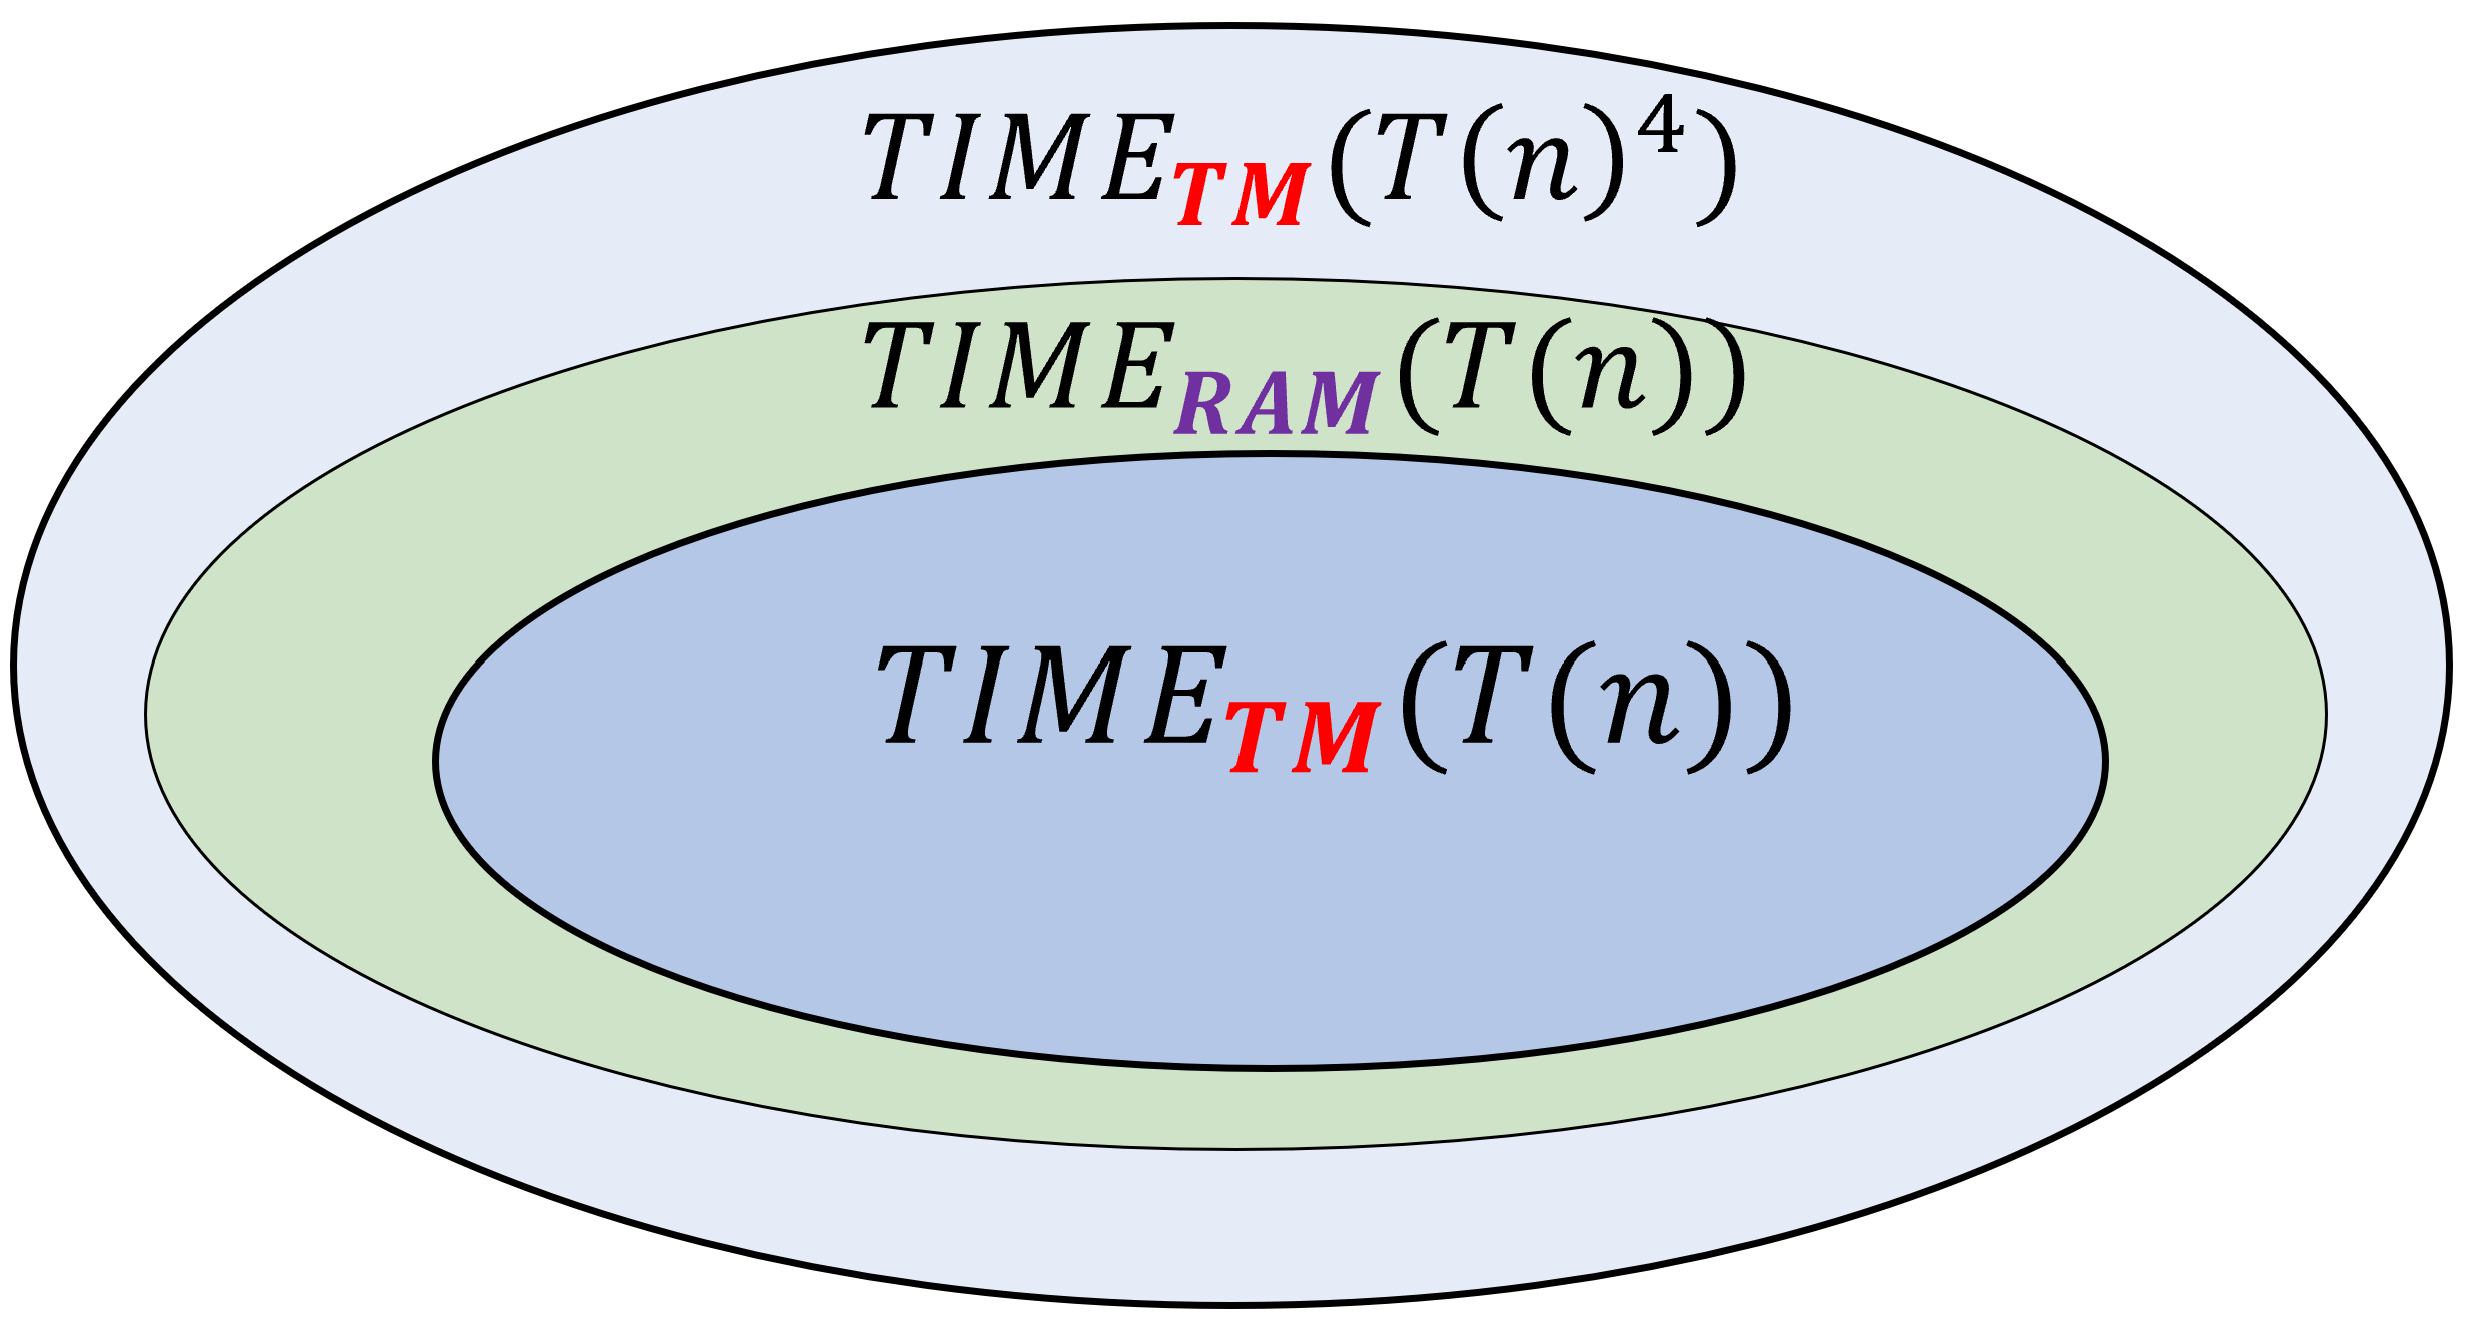
\includegraphics[width=\linewidth, height=1.5in, keepaspectratio]{../figure/RAMTMsimulation.png}
\caption{The proof of \cref{polyRAMTM-thm} shows that we can simulate
\(T\) steps of a Turing Machine with \(T\) steps of a NAND-RAM program,
and can simulate \(T\) steps of a NAND-RAM program with \(o(T^4)\) steps
of a Turing Machine. Hence
\(\ensuremath{\mathit{TIME}}_{\mathsf{TM}}(T(n)) \subseteq \ensuremath{\mathit{TIME}}_{\mathsf{RAM}}(10\cdot T(n)) \subseteq \ensuremath{\mathit{TIME}}_{\mathsf{TM}}(T(n)^4)\).}
\label{RAMTMsimulationfig}
\end{marginfigure}

For example, by instantiating \cref{polyRAMTM-thm} with \(T(n)=n^a\) and
using the fact that \(10n^a = o(n^{a+1})\), we see that
\(\ensuremath{\mathit{TIME}}_{\mathsf{TM}}(n^a) \subseteq \ensuremath{\mathit{TIME}}_{\mathsf{RAM}}(n^{a+1}) \subseteq \ensuremath{\mathit{TIME}}_{\mathsf{TM}}(n^{4a+4})\)
which means that (by \cref{diffdefofP}) \[
\mathbf{P} = \cup_{a = 1,2,\ldots} \ensuremath{\mathit{TIME}}_{\mathsf{TM}}(n^a) = \cup_{a = 1,2,\ldots} \ensuremath{\mathit{TIME}}_{\mathsf{RAM}}(n^a) \;.
\] That is, we could have equally well defined \(\mathbf{P}\) as the
class of functions computable by \emph{NAND-RAM programs} (instead of
Turing Machines) that run in time polynomial in the length of the input.
Similarly, by instantiating \cref{polyRAMTM-thm} with \(T(n)=2^{n^a}\)
we see that the class \(\mathbf{EXP}\) can also be defined as the set of
functions computable by NAND-RAM programs in time at most \(2^{p(n)}\)
where \(p\) is some polynomial. Similar equivalence results are known
for many models including cellular automata, C/Python/Javascript
programs, parallel computers, and a great many other models, which
justifies the choice of \(\mathbf{P}\) as capturing a
technology-independent notion of tractability. (See \cref{ECTTsec} for
more discussion of this issue.) This equivalence between Turing machines
and NAND-RAM (as well as other models) allows us to pick our favorite
model depending on the task at hand (i.e., ``have our cake and eat it
too'') even when we study questions of efficiency, as long as we only
care about the gap between \emph{polynomial} and \emph{exponential}
time. When we want to \emph{design} an algorithm, we can use the extra
power and convenience afforded by NAND-RAM. When we want to
\emph{analyze} a program or prove a \emph{negative result}, we can
restrict our attention to Turing machines.

\hypertarget{polyvsnot}{}
\begin{bigidea} \label[bigidea]{polyvsnot}

All ``reasonable'' computational models are equivalent if we only care
about the distinction between polynomial and exponential.

\end{bigidea}

The adjective ``reasonable'' above refers to all scalable computational
models that have been implemented, with the possible exception of
\emph{quantum computers}, see \cref{ECTTsec} and \cref{quantumchap}.

\begin{proofidea} \label[proofidea]{The-direction-ensuremathm}

The direction
\(\ensuremath{\mathit{TIME}}_{\mathsf{TM}}(T(n)) \subseteq \ensuremath{\mathit{TIME}}_{\mathsf{RAM}}(10 \cdot T(n))\)
is not hard to show, since a NAND-RAM program \(P\) can simulate a
Turing Machine \(M\) with constant overhead by storing the transition
table of \(M\) in an array (as is done in the proof of
\cref{universaltmthm}). Simulating every step of the Turing machine can
be done in a constant number \(c\) of steps of RAM, and it can be shown
this constant \(c\) is smaller than \(10\). Thus the heart of the
theorem is to prove that
\(\ensuremath{\mathit{TIME}}_{\mathsf{RAM}}(T(n)) \subseteq \ensuremath{\mathit{TIME}}_{\mathsf{TM}}(T(n)^4)\).
This proof closely follows the proof of \cref{RAMTMequivalencethm},
where we have shown that every function \(F\) that is computable by a
NAND-RAM program \(P\) is computable by a Turing Machine (or
equivalently a NAND-TM program) \(M\). To prove \cref{polyRAMTM-thm}, we
follow the exact same proof but just check that the overhead of the
simulation of \(P\) by \(M\) is polynomial. The proof has many details,
but is not deep. It is therefore much more important that you understand
the \emph{statement} of this theorem than its proof.

\end{proofidea}

\begin{proof}[Proof of \cref{polyRAMTM-thm}] \label[proof]{We-only-focus-on-the-non-}

We only focus on the non-trivial direction
\(\ensuremath{\mathit{TIME}}_{\mathsf{RAM}}(T(n)) \subseteq \ensuremath{\mathit{TIME}}_{\mathsf{TM}}(T(n)^4)\).
Let \(F\in \ensuremath{\mathit{TIME}}_{\mathsf{RAM}}(T(n))\). \(F\) can
be computed in time \(T(n)\) by some NAND-RAM program \(P\) and we need
to show that it can also be computed in time \(T(n)^4\) by a Turing
Machine \(M\). This will follow from showing that \(F\) can be computed
in time \(T(n)^4\) by a NAND-TM program, since for every NAND-TM program
\(Q\) there is a Turing Machine \(M\) simulating it such that each
iteration of \(Q\) corresponds to a single step of \(M\).

As mentioned above, we follow the proof of \cref{RAMTMequivalencethm}
(simulation of NAND-RAM programs using NAND-TM programs) and use the
exact same simulation, but with a more careful accounting of the number
of steps that the simulation costs. Recall, that the simulation of
NAND-RAM works by ``peeling off'' features of NAND-RAM one by one, until
we are left with NAND-TM.

We will not provide the full details but will present the main ideas
used in showing that every feature of NAND-RAM can be simulated by
NAND-TM with at most a polynomial overhead:

\begin{enumerate}
\def\labelenumi{\arabic{enumi}.}
\item
  Recall that every NAND-RAM variable or array element can contain an
  integer between \(0\) and \(T\) where \(T\) is the number of lines
  that have been executed so far. Therefore if \(P\) is a NAND-RAM
  program that computes \(F\) in \(T(n)\) time, then on inputs of length
  \(n\), all integers used by \(P\) are of magnitude at most \(T(n)\).
  This means that the largest value \texttt{i} can ever reach is at most
  \(T(n)\) and so each one of \(P\)'s variables can be thought of as an
  array of at most \(T(n)\) indices, each of which holds a natural
  number of magnitude at most \(T(n)\). We let
  \(\ell = \ceil{\log T(n)}\) be the number of bits needed to encode
  such numbers. (We can start off the simulation by computing \(T(n)\)
  and \(\ell\).)
\item
  We can encode a NAND-RAM array of length \(\leq T(n)\) containing
  numbers in \(\{0,\ldots, T(n)-1 \}\) as an Boolean (i.e., NAND-TM)
  array of \(T(n)\ell =O(T(n)\log T(n))\) bits, which we can also think
  of as a \emph{two dimensional array} as we did in the proof of
  \cref{RAMTMequivalencethm}. We encode a NAND-RAM scalar containing a
  number in \(\{0,\ldots, T(n)-1 \}\) simply by a shorter NAND-TM array
  of \(\ell\) bits.
\item
  We can simulate the two dimensional arrays using one-dimensional
  arrays of length \(T(n)\ell = O(T(n) \log T(n)\). All the arithmetic
  operations on integers use the grade-school algorithms, that take time
  that is polynomial in the number \(\ell\) of bits of the integers,
  which is \(poly(\log T(n))\) in our case. Hence we can simulate
  \(T(n)\) steps of NAND-RAM with \(O(T(n)poly(\log T(n))\) steps of a
  model that uses random access memory but only \emph{Boolean-valued}
  one-dimensional arrays.
\item
  The most expensive step is to translate from random access memory to
  the sequential memory model of NAND-TM/Turing Machines. As we did in
  the proof of \cref{RAMTMequivalencethm} (see
  \cref{nandtmgorydetailssec}), we can simulate accessing an array
  \texttt{Foo} at some location encoded in an array \texttt{Bar} by:

  \begin{enumerate}
  \def\labelenumii{\alph{enumii}.}
  \tightlist
  \item
    Copying \texttt{Bar} to some temporary array \texttt{Temp}
  \item
    Having an array \texttt{Index} which is initially all zeros except
    \(1\) at the first location.
  \item
    Repeating the following until \texttt{Temp} encodes the number
    \(0\): \emph{(Number of repetitions is at most \(T(n)\).)}

    \begin{itemize}
    \tightlist
    \item
      Decrease the number encoded temp by \(1\). \emph{(Take number of
      steps polynomial in \(\ell = \ceil{\log T(n)}\).)}
    \item
      Decrease \texttt{i} until it is equal to \(0\). \emph{(Take
      \(O(T(n)\) steps.)}
    \item
      Scan \texttt{Index} until we reach the point in which it equals
      \(1\) and then change this \(1\) to \(0\) and go one step further
      and write \(1\) in this location. \emph{(Takes \(O(T(n))\)
      steps.)}
    \end{itemize}
  \item
    When we are done we know that if we scan \texttt{Index} until we
    reach the point in which \texttt{Index[i]}\(=1\) then \texttt{i}
    contains the value that was encoded by \texttt{Bar} \emph{(Takes
    \(O(T(n)\) steps.)}
  \end{enumerate}
\end{enumerate}

The total cost for each such operation is
\(O(T(n)^2 + T(n)poly(\log T(n))) = O(T(n)^2)\) steps.

In sum, we simulate a single step of NAND-RAM using
\(O(T(n)^2 poly(\log T(n)))\) steps of NAND-TM, and hence the total
simulation time is \(O(T(n)^3 poly(\log T(n)))\) which is smaller than
\(T(n)^4\) for sufficiently large \(n\).

\end{proof}

\hypertarget{nicefunctionsrem}{}
\begin{remark}[Nice time bounds] \label[remark]{nicefunctionsrem}

When considering general time bounds such we need to make sure to rule
out some ``pathological'' cases such as functions \(T\) that don't give
enough time for the algorithm to read the input, or functions where the
time bound itself is uncomputable. We say that a function
\(T:\N \rightarrow \N\) is a \emph{nice time bound function} (or nice
function for short) if for every \(n\in \N\), \(T(n) \geq n\) (i.e.,
\(T\) allows enough time to read the input), for every \(n' \geq n\),
\(T(n') \geq T(n)\) (i.e., \(T\) allows more time on longer inputs), and
the map \(F(x) = 1^{T(|x|)}\) (i.e., mapping a string of length \(n\) to
a sequence of \(T(n)\) ones) can be computed by a NAND-RAM program in
\(O(T(n))\) time.

All the ``normal'' time complexity bounds we encounter in applications
such as \(T(n)= 100 n\), \(T(n) = n^2 \log n\),\(T(n) = 2^{\sqrt{n}}\),
etc. are ``nice''. Hence from now on we will only care about the class
\(\ensuremath{\mathit{TIME}}(T(n))\) when \(T\) is a ``nice'' function.
The computability condition is in particular typically easily satisfied.
For example, for arithmetic functions such as \(T(n) = n^3\), we can
typically compute the binary representation of \(T(n)\) in time
polynomial \emph{in the number of bits} of \(T(n)\) and hence
poly-logarithmic in \(T(n)\). Hence the time to write the string
\(1^{T(n)}\) in such cases will be \(T(n) + poly(\log T(n)) = O(T(n))\).

\end{remark}

\section{Extended Church-Turing Thesis (discussion)}\label{ECTTsec}

\cref{polyRAMTM-thm} shows that the computational models of \emph{Turing
Machines} and \emph{RAM Machines / NAND-RAM programs} are equivalent up
to polynomial factors in the running time. Other examples of
polynomially equivalent models include:

\begin{itemize}
\item
  All standard programming languages, including
  C/Python/JavaScript/Lisp/etc.
\item
  The \(\lambda\) calculus (see also \cref{bibnotesrunningtime}).
\item
  Cellular automata
\item
  Parallel computers
\item
  Biological computing devices such as DNA-based computers.
\end{itemize}

The \emph{Extended Church Turing Thesis} is the statement this is true
for all physically realizable computing models. In other words, the
extended Church Turing thesis says that for every \emph{scalable
computing device} \(C\) (which has a finite description but can be in
principle used to run computation on arbitrarily large inputs), there is
some constant \(a\) such that for every function
\(F:\{0,1\}^* \rightarrow \{0,1\}\) that \(C\) can compute on \(n\)
length inputs using an \(S(n)\) amount of physical resources, \(F\) is
in \(\ensuremath{\mathit{TIME}}(S(n)^a)\). This is a strengthening of
the (``plain'') Church-Turing Thesis, discussed in
\cref{churchturingdiscussionsec}, which states that the set of
computable functions is the same for all physically realizable models,
but without requiring the overhead in the simulation between different
models to be at most polynomial.

All the current constructions of scalable computational models and
programming language conform to the Extended Church-Turing Thesis, in
the sense that they can be with polynomial overhead by Turing Machines
(and hence also by NAND-TM or NAND-RAM programs). consequently, the
classes \(\mathbf{P}\) and \(\mathbf{EXP}\) are robust to the choice of
model, and we can use the programming language of our choice, or high
level descriptions of an algorithm, to determine whether or not a
problem is in \(\mathbf{P}\).

Like the Church-Turing thesis itself, the extended Church-Turing thesis
is in the asymptotic setting and does not directly yield an
experimentally testable prediction. However, it can be instantiated with
more concrete bounds on the overhead, yielding experimentally-testable
predictions such as the \emph{Physical Extended Church-Turing Thesis} we
mentioned in \cref{PECTTsec}.

In the last hundred+ years of studying and mechanizing computation, no
one has yet constructed a scalable computing device that violates the
extended Church Turing Thesis. However, \emph{quantum computing}, if
realized, will pose a serious challenge to the extended Church-Turing
Thesis (see \cref{quantumchap}). However, even if the promises of
quantum computing are fully realized, the extended Church-Turing thesis
is ``morally'' correct, in the sense that, while we do need to adapt the
thesis to account for the possibility of quantum computing, its broad
outline remains unchanged. We are still able to model computation
mathematically, we can still treat programs as strings and have a
universal program, we still have time hierarchy and uncomputability
results, and there is still no reason to doubt the (``plain'')
Church-Turing thesis. Moreover, the prospect of quantum computing does
not seem to make a difference for the time complexity of many (though
not all!) of the concrete problems that we care about. In particular, as
far as we know, out of all the example problems mentioned in
\cref{chapefficient} the complexity of only one--- integer factoring---
is affected by modifying our model to include quantum computers as well.

\section{Efficient universal machine: a NAND-RAM interpreter in
NAND-RAM}\label{Efficient-universal-machi}

We have seen in \cref{universaltmthm} the ``universal Turing Machine''.
Examining that proof, and combining it with \cref{polyRAMTM-thm} , we
can see that the program \(U\) has a \emph{polynomial} overhead, in the
sense that it can simulate \(T\) steps of a given NAND-TM (or NAND-RAM)
program \(P\) on an input \(x\) in \(O(T^4)\) steps. But in fact, by
directly simulating NAND-RAM programs we can do better with only a
\emph{constant} multiplicative overhead. That is, there is a
\emph{universal NAND-RAM program} \(U\) such that for every NAND-RAM
program \(P\), \(U\) simulates \(T\) steps of \(P\) using only \(O(T)\)
steps. (The implicit constant in the \(O\) notation can depend on the
program \(P\) but does \emph{not} depend on the length of the input.)

\hypertarget{univ-nandpp}{}
\begin{theorem}[Efficient universality of NAND-RAM] \label[theorem]{univ-nandpp}

There exists a NAND-RAM program \(U\) satisfying the following:

\begin{enumerate}
\def\labelenumi{\arabic{enumi}.}
\item
  \emph{(\(U\) is a universal NAND-RAM program.)} For every NAND-RAM
  program \(P\) and input \(x\), \(U(P,x)=P(x)\) where by \(U(P,x)\) we
  denote the output of \(U\) on a string encoding the pair \((P,x)\).
\item
  \emph{(\(U\) is efficient.)} There are some constants \(a,b\) such
  that for every NAND-RAM program \(P\), if \(P\) halts on input \(x\)
  after most \(T\) steps, then \(U(P,x)\) halts after at most
  \(C\cdot T\) steps where \(C \leq a |P|^b\).
\end{enumerate}

\end{theorem}

\begin{pause} \label[pause]{As-in-the-case-of-crefpol}

As in the case of \cref{polyRAMTM-thm}, the proof of \cref{univ-nandpp}
is not very deep and so it is more important to understand its
\emph{statement}. Specifically, if you understand how you would go about
writing an interpreter for NAND-RAM using a modern programming language
such as Python, then you know everything you need to know about the
proof of this theorem.

\end{pause}


\begin{marginfigure}
\centering
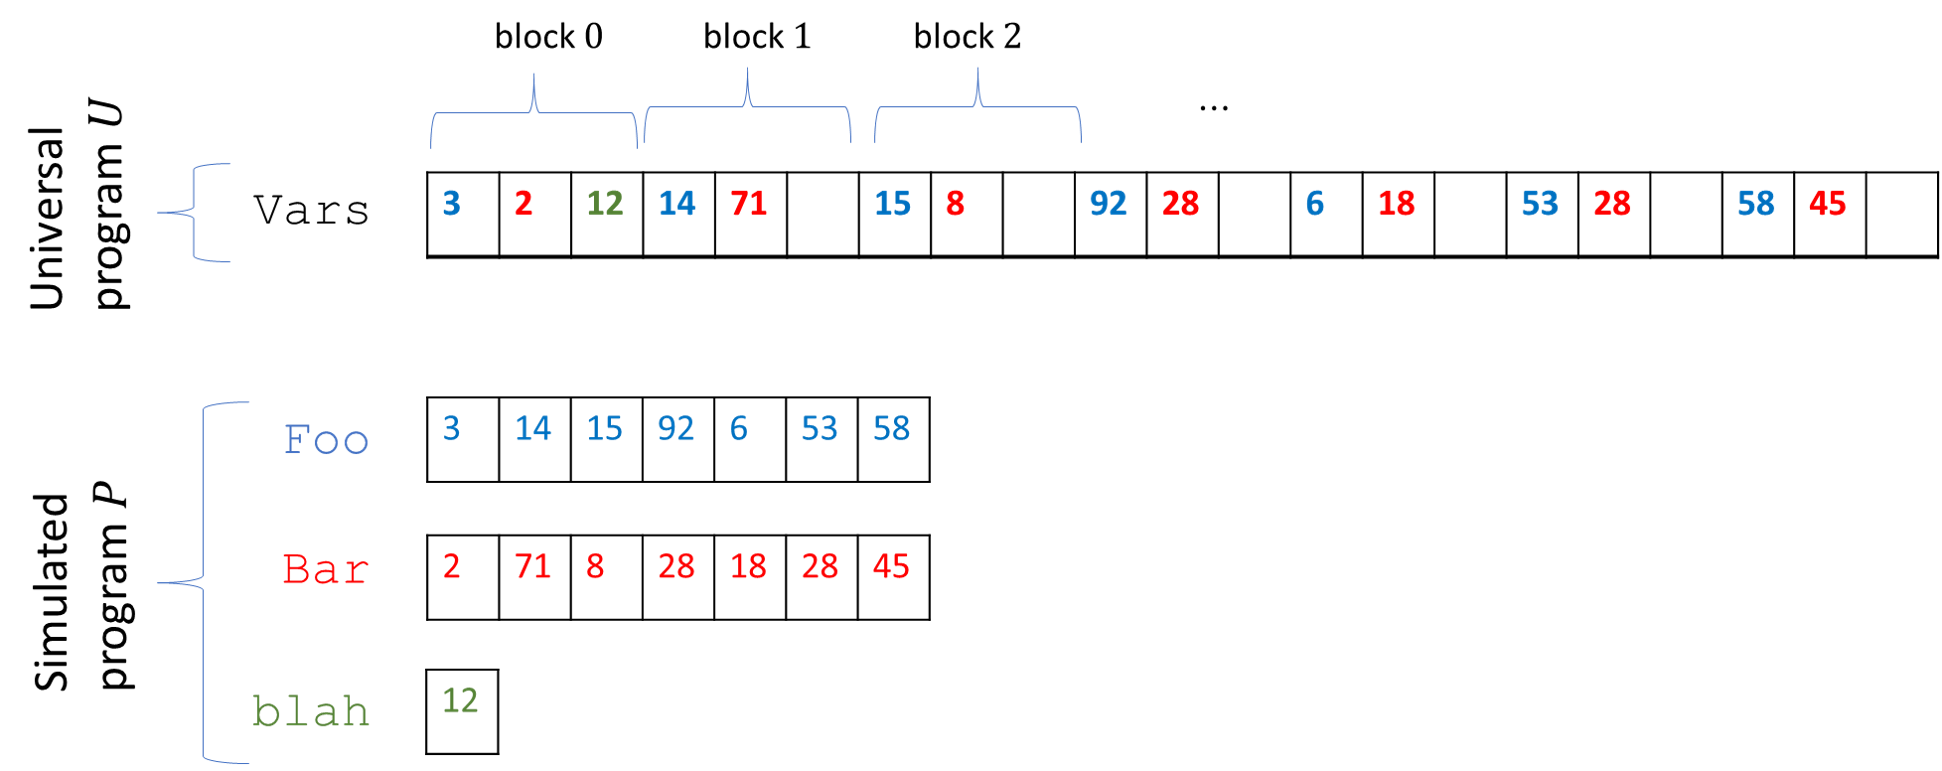
\includegraphics[width=\linewidth, height=1.5in, keepaspectratio]{../figure/universalrammachine.png}
\caption{The universal NAND-RAM program \(U\) simulates an input
NAND-RAM program \(P\) by storing all of \(P\)'s variables inside a
single array \texttt{Vars} of \(U\). If \(P\) has \(t\) variables, then
the array \texttt{Vars} is divided into blocks of length \(t\), where
the \(j\)-th coordinate of the \(i\)-th block contains the \(i\)-th
element of the \(j\)-th array of \(P\). If the \(j\)-th variable of
\(P\) is scalar, then we just store its value in the zeroth block of
\texttt{Vars}.}
\label{universalrammachinefig}
\end{marginfigure}

\begin{proof}[Proof of \cref{univ-nandpp}] \label[proof]{To-present-a-universal-NA}

To present a universal NAND-RAM program in full we would need to
describe a precise representation scheme, as well as the full NAND-RAM
instructions for the program. While this can be done, it is more
important to focus on the main ideas, and so we just sketch the proof
here. A specification of NAND-RAM is given in the
\href{http://tiny.cc/introtcsappendix}{appendix}, and for the purposes
of this simulation, we can simply use the representation of the code
NAND-RAM as an ASCII string.

The program \(U\) gets as input a NAND-RAM program \(P\) and an input
\(x\) and simulates \(P\) one step at a time. To do so, \(U\) does the
following:

\begin{enumerate}
\def\labelenumi{\arabic{enumi}.}
\item
  \(U\) maintains variables \texttt{program\_counter}, and
  \texttt{number\_steps} for the current line to be executed and the
  number of steps executed so far.
\item
  \(U\) initially scans the code of \(P\) to find the number \(t\) of
  unique variable names that \(P\) uses. It will translate each variable
  name into a number between \(0\) and \(t-1\) and use an array
  \texttt{Program} to store \(P\)'s code where for every line \(\ell\),
  \texttt{Program[}\(\ell\)\texttt{]} will store the \(\ell\)-th line of
  \(P\) where the variable names have been translated to numbers. (More
  concretely, we will use a constant number of arrays to separately
  encode the operation used in this line, and the variable names and
  indices of the operands.)
\item
  \(U\) maintains a single array \texttt{Vars} that contains all the
  values of \(P\)'s variables. We divide \texttt{Vars} into blocks of
  length \(t\). If \(s\) is a number corresponding to an array variable
  \texttt{Foo} of \(P\), then we store \texttt{Foo[0]} in
  \texttt{Vars[}\(s\)\texttt{]}, we store \texttt{Foo[1]} in
  \texttt{Var\_values[}\(t+s\)\texttt{]}, \texttt{Foo[2]} in
  \texttt{Vars[}\(2t + s\)\texttt{]} and so on and so forth (see
  \cref{universalrammachinefig}). Generally,if the \(s\)-th variable of
  \(P\) is a scalar variable, then its value will be stored in location
  \texttt{Vars[}\(s\)\texttt{]}. If it is an array variable then the
  value of its \(i\)-th element will be stored in location
  \texttt{Vars[}\(t\cdot i + s\)\texttt{]}.
\item
  To simulate a single step of \(P\), the program \(U\) recovers from
  \texttt{Program} the line corresponding to \texttt{program\_counter}
  and executes it. Since NAND-RAM has a constant number of arithmetic
  operations, we can implement the logic of which operation to execute
  using a sequence of a constant number of if-then-else's. Retrieving
  from \texttt{Vars} the values of the operands of each instruction can
  be done using a constant number of arithmetic operations.
\end{enumerate}

The setup stages take only a constant (depending on \(|P|\) but not on
the input \(x\)) number of steps. Once we are done with the setup, to
simulate a single step of \(P\), we just need to retrieve the
corresponding line and do a constant number of ``if elses'' and accesses
to \texttt{Vars} to simulate it. Hence the total running time to
simulate \(T\) steps of the program \(P\) is at most \(O(T)\) when
suppressing constants that depend on the program \(P\).

\end{proof}

\subsection{Timed Universal Turing
Machine}\label{Timed-Universal-Turing-Ma}

One corollary of the efficient universal machine is the following. Given
any Turing Machine \(M\), input \(x\), and ``step budget'' \(T\), we can
simulate the execution of \(M\) for \(T\) steps in time that is
polynomial in \(T\). Formally, we define a function
\(\ensuremath{\mathit{TIMEDEVAL}}\) that takes the three parameters
\(M\), \(x\), and the time budget, and outputs \(M(x)\) if \(M\) halts
within at most \(T\) steps, and outputs \(0\) otherwise. The timed
universal Turing Machine computes \(\ensuremath{\mathit{TIMEDEVAL}}\) in
polynomial time (see \cref{timeduniversaltmfig}). (Since we measure time
as a function of the input length, we define
\(\ensuremath{\mathit{TIMEDEVAL}}\) as taking the input \(T\)
represented in \emph{unary}: a string of \(T\) ones.)

\hypertarget{timeduniversalTM}{}
\begin{theorem}[Timed Universal Turing Machine] \label[theorem]{timeduniversalTM}

Let \(\ensuremath{\mathit{TIMEDEVAL}}:\{0,1\}^* \rightarrow \{0,1\}^*\)
be the function defined as
\[\ensuremath{\mathit{TIMEDEVAL}}(M,x,1^T) = \begin{cases} M(x) & M \text{ halts within $\leq T$ steps on $x$} \\ 0 & \text{otherwise}\end{cases} \;.\]
Then \(\ensuremath{\mathit{TIMEDEVAL}} \in \mathbf{P}\).

\end{theorem}


\begin{marginfigure}
\centering
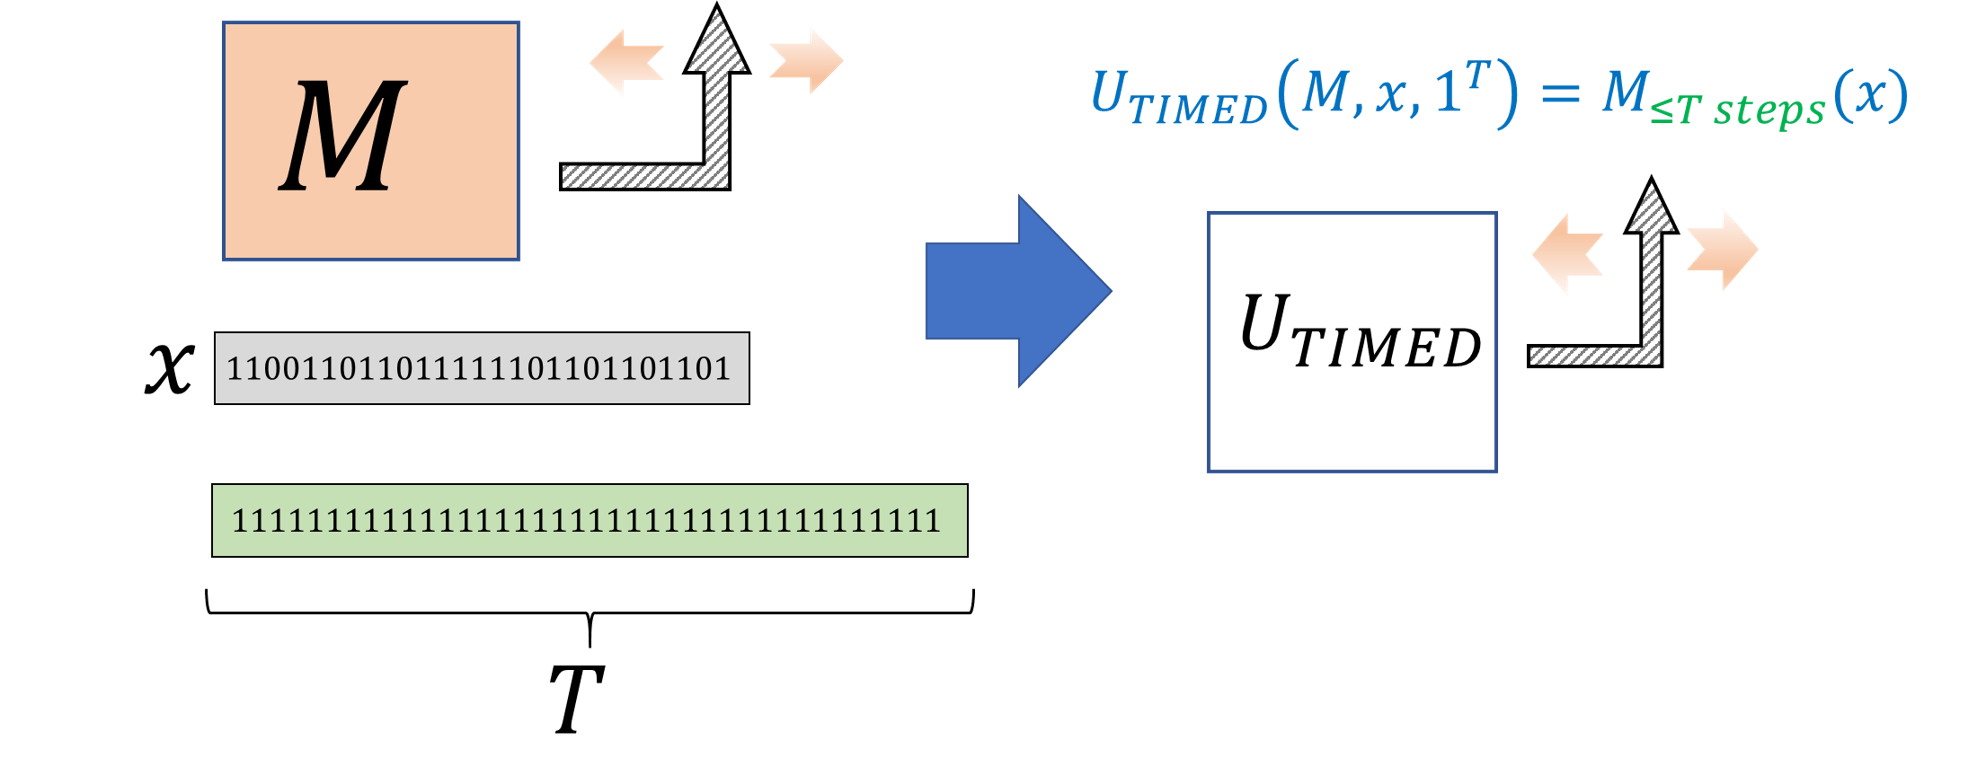
\includegraphics[width=\linewidth, height=1.5in, keepaspectratio]{../figure/timeduniversaltm.png}
\caption{The \emph{timed} universal Turing Machine takes as input a
Turing machine \(M\), an input \(x\), and a time bound \(T\), and
outputs \(M(x)\) if \(M\) halts within at most \(T\) steps.
\cref{timeduniversalTM}states that there is such a machine that runs in
time polynomial in \(T\).}
\label{timeduniversaltmfig}
\end{marginfigure}

\begin{proof} \label[proof]{We-only-sketch-the-proof-}

We only sketch the proof since the result follows fairly directly from
\cref{polyRAMTM-thm} and \cref{univ-nandpp}. By \cref{polyRAMTM-thm} to
show that \(\ensuremath{\mathit{TIMEDEVAL}} \in \mathbf{P}\), it
suffices to give a polynomial-time NAND-RAM program to compute
\(\ensuremath{\mathit{TIMEDEVAL}}\).

Such a program can be obtained as follows. Given a Turing Machine \(M\),
by \cref{polyRAMTM-thm} we can transform it in time polynomial in its
description into a functionally-equivalent NAND-RAM program \(P\) such
that the execution of \(M\) on \(T\) steps can be simulated by the
execution of \(P\) on \(c\cdot T\) steps. We can then run the universal
NAND-RAM machine of \cref{univ-nandpp} to simulate \(P\) for
\(c\cdot T\) steps, using \(O(T)\) time, and output \(0\) if the
execution did not halt within this budget. This shows that
\(\ensuremath{\mathit{TIMEDEVAL}}\) can be computed by a NAND-RAM
program in time polynomial in \(|M|\) and linear in \(T\), which means
\(\ensuremath{\mathit{TIMEDEVAL}} \in \mathbf{P}\).

\end{proof}

\section{The time hierarchy theorem}\label{The-time-hierarchy-theore}

Some functions are \emph{uncomputable}, but are there functions that can
be computed, but only at an exorbitant cost? For example, is there a
function that \emph{can} be computed in time \(2^n\), but \emph{can not}
be computed in time \(2^{0.9 n}\)? It turns out that the answer is
\textbf{Yes}:

\hypertarget{time-hierarchy-thm}{}
\begin{theorem}[Time Hierarchy Theorem] \label[theorem]{time-hierarchy-thm}

For every nice function \(T:\N \rightarrow \N\), there is a function
\(F:\{0,1\}^* \rightarrow \{0,1\}\) in
\(\ensuremath{\mathit{TIME}}(T(n)\log n) \setminus \ensuremath{\mathit{TIME}}(T(n))\).

\end{theorem}

There is nothing special about \(\log n\), and we could have used any
other efficiently computable function that tends to infinity with \(n\).

\hypertarget{timehierarchy}{}
\begin{bigidea} \label[bigidea]{timehierarchy}

If we have more time, we can compute more functions.

\end{bigidea}

\hypertarget{hierarchytoyrem}{}
\begin{remark}[Simpler corollary of the time hierarchy theorem] \label[remark]{hierarchytoyrem}

The generality of the time hierarchy theorem can make its proof a little
hard to read. It might be easier to follow the proof if you first try to
prove by yourself the easier statement
\(\mathbf{P} \subsetneq \mathbf{EXP}\).

You can do so by showing that the following function
\(F:\{0,1\}^* :\rightarrow \{0,1\}\) is in
\(\mathbf{EXP} \setminus \mathbf{P}\): for every Turing Machine \(M\)
and input \(x\), \(F(M,x)=1\) if and only if \(M\) halts on \(x\) within
at most \(|x|^{\log |x|}\) steps. One can show that
\(F \in \ensuremath{\mathit{TIME}}(n^{O(\log n)}) \subseteq \mathbf{EXP}\)
using the universal Turing machine (or the efficient universal NAND-RAM
program of \cref{univ-nandpp}). On the other harnd, we can use similar
ideas to those used to show the uncomputability of
\(\ensuremath{\mathit{HALT}}\) in \cref{haltalternativesec} to prove
that \(F \not\in \mathbf{P}\).

\end{remark}


\begin{figure}
\centering
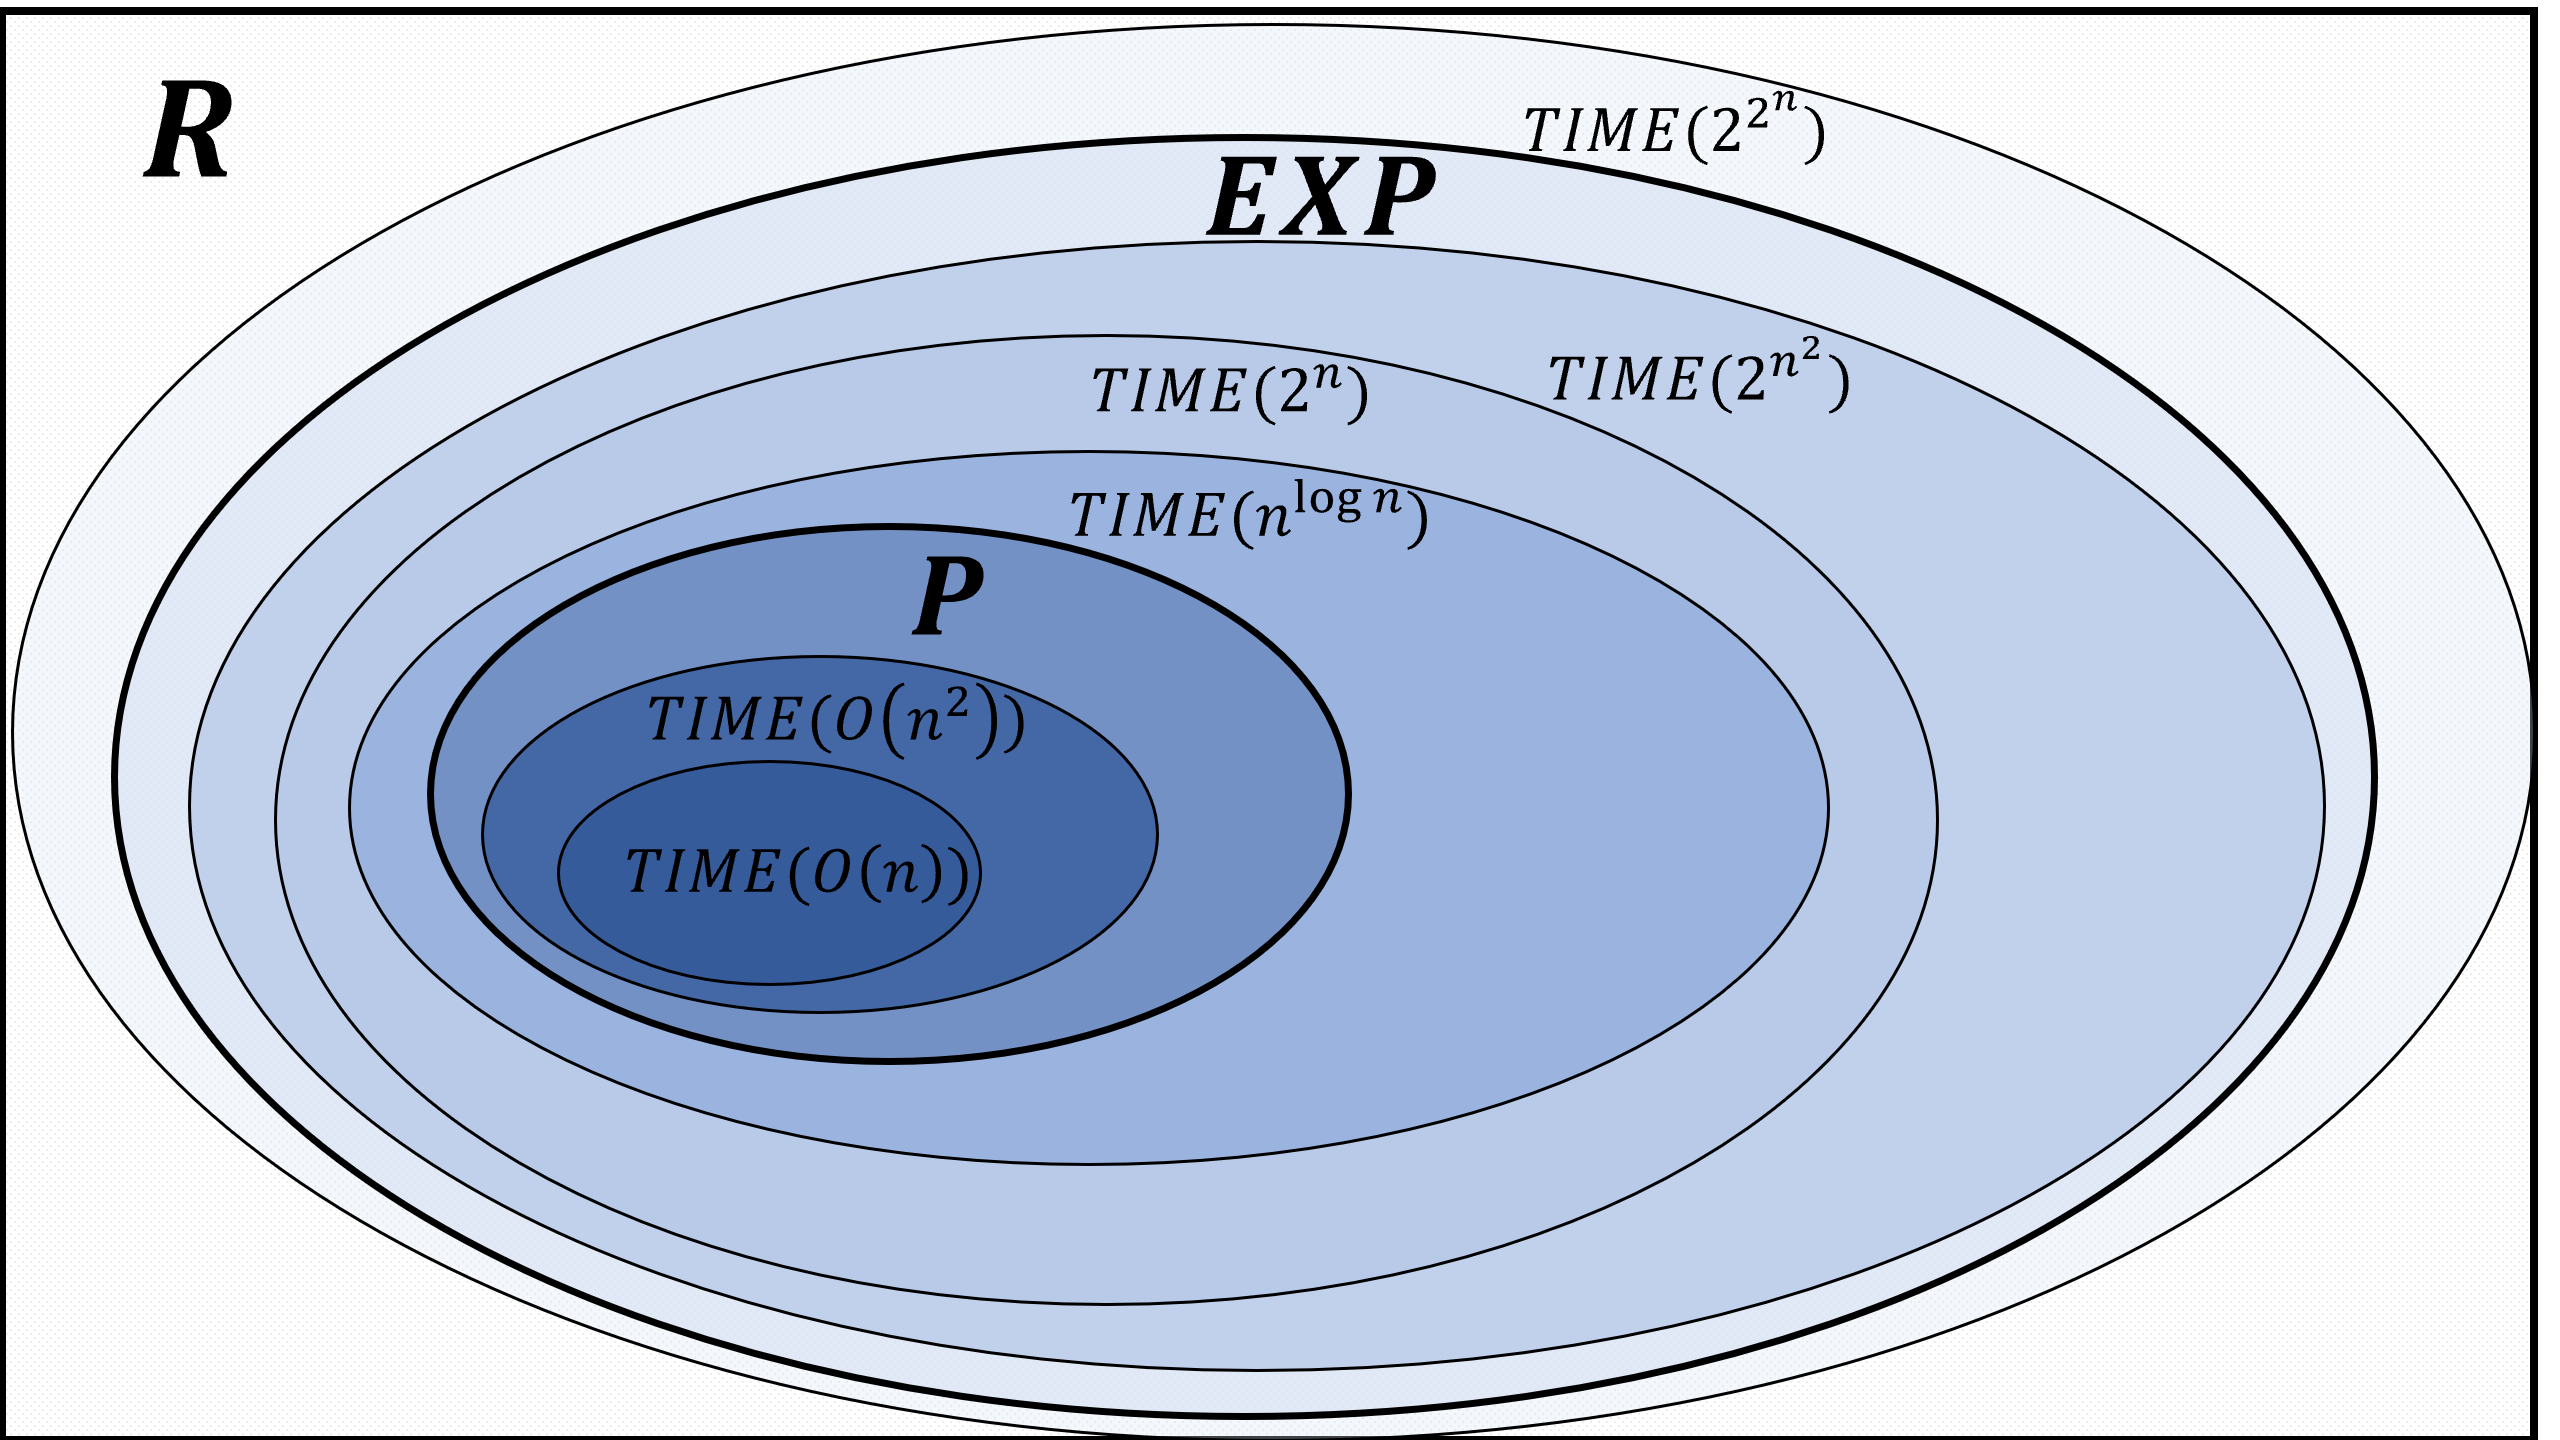
\includegraphics[width=\textwidth, height=0.25\paperheight, keepaspectratio]{../figure/timehierarchythm.png}
\caption{The \emph{Time Hierarchy Theorem} (\cref{time-hierarchy-thm})
states that all of these classes are \emph{distinct}.}
\label{timehierarchythmfig}
\end{figure}

\begin{proofidea} \label[proofidea]{In-the-proof-of-crefhalt-}

In the proof of \cref{halt-thm} (the uncomputability of the Halting
problem), we have shown that the function \(\ensuremath{\mathit{HALT}}\)
cannot be computed in any finite time. An examination of the proof shows
that it gives something stronger. Namely, the proof shows that if we fix
our computational budget to be \(T\) steps, then not only we can't
distinguish between programs that halt and those that do not, but cannot
even distinguish between programs that halt within at most \(T'\) steps
and those that take more than that (where \(T'\) is some number
depending on \(T\)). Therefore, the proof of \cref{time-hierarchy-thm}
follows the ideas of the uncomputability of the halting problem, but
again with a more careful accounting of the running time.

\end{proofidea}

\begin{proof}[Proof of \cref{time-hierarchy-thm}] \label[proof]{Our-proof-is-inspired-by-}

Our proof is inspired by the proof of the uncomputability of the halting
problem. Specifically, for every function \(T\) as in the theorem's
statement, we define the \emph{Bounded Halting} function
\(\ensuremath{\mathit{HALT}}_T\) as follows. The input to
\(\ensuremath{\mathit{HALT}}_T\) is a pair \((P,x)\) such that
\(|P| \leq \log \log |x|\) encodes some NAND-RAM program. We define

\[
\ensuremath{\mathit{HALT}}_T(P,x) = \begin{cases}1, & P \text{ halts on } x \text{ within } \leq 100\cdot T(|P|+|x|) \text{ steps} \\
0, & \text{otherwise} \end{cases} \;.
\] (The constant \(100\) and the function \(\log \log n\) are rather
arbitrary, and are chosen for convenience in this proof.)

\cref{time-hierarchy-thm} is an immediate consequence of the following
two claims:

\textbf{Claim 1:}
\(\ensuremath{\mathit{HALT}}_T \in \ensuremath{\mathit{TIME}}(T(n)\cdot \log n)\)

and

\textbf{Claim 2:}
\(\ensuremath{\mathit{HALT}}_T \not\in \ensuremath{\mathit{TIME}}(T(n))\).

Please make sure you understand why indeed the theorem follows directly
from the combination of these two claims. We now turn to proving them.

\textbf{Proof of claim 1:} We can easily check in linear time whether an
input has the form \(P,x\) where \(|P| \leq \log\log |x|\). Since
\(T(\cdot)\) is a nice function, we can evaluate it in \(O(T(n))\) time.
Thus, we can compute \(\ensuremath{\mathit{HALT}}_T(P,x)\) as follows:

\begin{enumerate}
\def\labelenumi{\arabic{enumi}.}
\item
  Compute \(T_0=T(|P|+|x|)\) in \(O(T_0)\) steps.
\item
  Use the universal NAND-RAM program of \cref{univ-nandpp} to simulate
  \(100\cdot T_0\) steps of \(P\) on the input \(x\) using at most
  \(poly(|P|)T_0\) steps. (Recall that we use \(poly(\ell)\) to denote a
  quantity that is bounded by \(a\ell^b\) for some constants \(a,b\).)
\item
  If \(P\) halts within these \(100\cdot T_0\) steps then output \(1\),
  else output \(0\).
\end{enumerate}

The length of the input is \(n=|P|+|x|\). Since \(|x| \leq n\) and
\((\log \log |x|)^b = o(\log |x|)\) for every \(b\), the running time
will be \(o(T(|P|+|x|) \log n)\) and hence the above algorithm
demonstrates that
\(\ensuremath{\mathit{HALT}}_T \in \ensuremath{\mathit{TIME}}(T(n)\cdot \log n)\),
completing the proof of Claim 1.

\textbf{Proof of claim 2:} This proof is the heart of
\cref{time-hierarchy-thm}, and is very reminiscent of the proof that
\(\ensuremath{\mathit{HALT}}\) is not computable. Assume, for the sake
of contradiction, that there is some NAND-RAM program \(P^*\) that
computes \(\ensuremath{\mathit{HALT}}_T(P,x)\) within \(T(|P|+|x|)\)
steps. We are going to show a contradiction by creating a program \(Q\)
and showing that under our assumptions, if \(Q\) runs for less than
\(T(n)\) steps when given (a padded version of) its own code as input
then it actually runs for more than \(T(n)\) steps and vice versa. (It
is worth re-reading the last sentence twice or thrice to make sure you
understand this logic. It is very similar to the direct proof of the
uncomputability of the halting problem where we obtained a contradiction
by using an assumed ``halting solver'' to construct a program that,
given its own code as input, halts if and only if it does not halt.)

We will define \(Q^*\) to be the program that on input a string \(z\)
does the following:

\begin{enumerate}
\def\labelenumi{\arabic{enumi}.}
\item
  If \(z\) does not have the form \(z=P1^m\) where \(P\) represents a
  NAND-RAM program and \(|P|< 0.1 \log\log m\) then return \(0\).
  (Recall that \(1^m\) denotes the string of \(m\) ones.)
\item
  Compute \(b= P^*(P,z)\) (at a cost of at most \(T(|P|+|z|)\) steps,
  under our assumptions).
\item
  If \(b=1\) then \(Q^*\) goes into an infinite loop, otherwise it
  halts.
\end{enumerate}

Let \(\ell\) be the length description of \(Q^*\) as a string, and let
\(m\) be larger than \(2^{2^{1000 \ell}}\). We will reach a
contradiction by splitting into cases according to whether or not
\(\ensuremath{\mathit{HALT}}_T(Q^*,Q^*1^m)\) equals \(0\) or \(1\).

On the one hand, if \(\ensuremath{\mathit{HALT}}_T(Q^*,Q^*1^m)=1\), then
under our assumption that \(P^*\) computes
\(\ensuremath{\mathit{HALT}}_T\), \(Q^*\) will go into an infinite loop
on input \(z=Q^*1^m\), and hence in particular \(Q^*\) does \emph{not}
halt within \(100 T(|Q^*|+m)\) steps on the input \(z\). But this
contradicts our assumption that
\(\ensuremath{\mathit{HALT}}_T(Q^*,Q^*1^m)=1\).

This means that it must hold that
\(\ensuremath{\mathit{HALT}}_T(Q^*,Q^*1^m)=0\). But in this case, since
we assume \(P^*\) computes \(\ensuremath{\mathit{HALT}}_T\), \(Q^*\)
does not do anything in phase 3 of its computation, and so the only
computation costs come in phases 1 and 2 of the computation. It is not
hard to verify that Phase 1 can be done in linear and in fact less than
\(5|z|\) steps. Phase 2 involves executing \(P^*\), which under our
assumption requires \(T(|Q^*|+m)\) steps. In total we can perform both
phases in less than \(10 T(|Q^*|+m)\) in steps, which by definition
means that \(\ensuremath{\mathit{HALT}}_T(Q^*,Q^*1^m)=1\), but this is
of course a contradiction. This completes the proof of Claim 2 and hence
of \cref{time-hierarchy-thm}.

\end{proof}

\hypertarget{PvsEXPexercise}{}
\begin{solvedexercise}[$\mathbf{P}$ vs $\mathbf{EXP}$] \label[solvedexercise]{PvsEXPexercise}

Prove that \(\mathbf{P} \subsetneq \mathbf{EXP}\).

\end{solvedexercise}

\begin{solution} \label[solution]{We-show-why-this-statemen}

We show why this statement follows from the time hierarchy theorem, but
it can be an instructive exercise to prove it directly, see
\cref{hierarchytoyrem}. We need to show that there exists
\(F \in \mathbf{EXP} \setminus \mathbf{P}\). Let \(T(n) = n^{\log n}\)
and \(T'(n) = n^{\log n / 2}\). Both are nice functions. Since
\(T(n)/T'(n) = \omega(\log n)\), by \cref{time-hierarchy-thm} there
exists some \(F\) in
\(\ensuremath{\mathit{TIME}}(T'(n)) \subsetneq \ensuremath{\mathit{TIME}}(T(n))\).
Since for sufficiently large \(n\), \(2^n > n^{\log n}\),
\(F \in \ensuremath{\mathit{TIME}}(2^n) \subseteq \mathbf{EXP}\). On the
other hand, \(F \not\in \mathbf{P}\). Indeed, suppose otherwise that
there was a constant \(c>0\) and a Turing Machine computing \(F\) on
\(n\)-length input in at most \(n^c\) steps for all sufficiently large
\(n\). Then since for \(n\) large enough \(n^c < n^{\log n/2}\), it
would have followed that
\(F \in \ensuremath{\mathit{TIME}}(n^{\log n /2})\) contradicting our
choice of \(F\).

\end{solution}

The time hierarchy theorem tells us that there are functions we can
compute in \(O(n^2)\) time but not \(O(n)\), in \(2^n\) time, but not
\(2^{\sqrt{n}}\), etc.. In particular there are most definitely
functions that we can compute in time \(2^n\) but not \(O(n)\). We have
seen that we have no shortage of natural functions for which the best
\emph{known} algorithm requires roughly \(2^n\) time, and that many
people have invested significant effort in trying to improve that.
However, unlike in the finite vs.~infinite case, for all of the examples
above at the moment we do not know how to rule out even an \(O(n)\) time
algorithm. We will however see that there is a single unproven
conjecture that would imply such a result for most of these problems.


\begin{marginfigure}
\centering
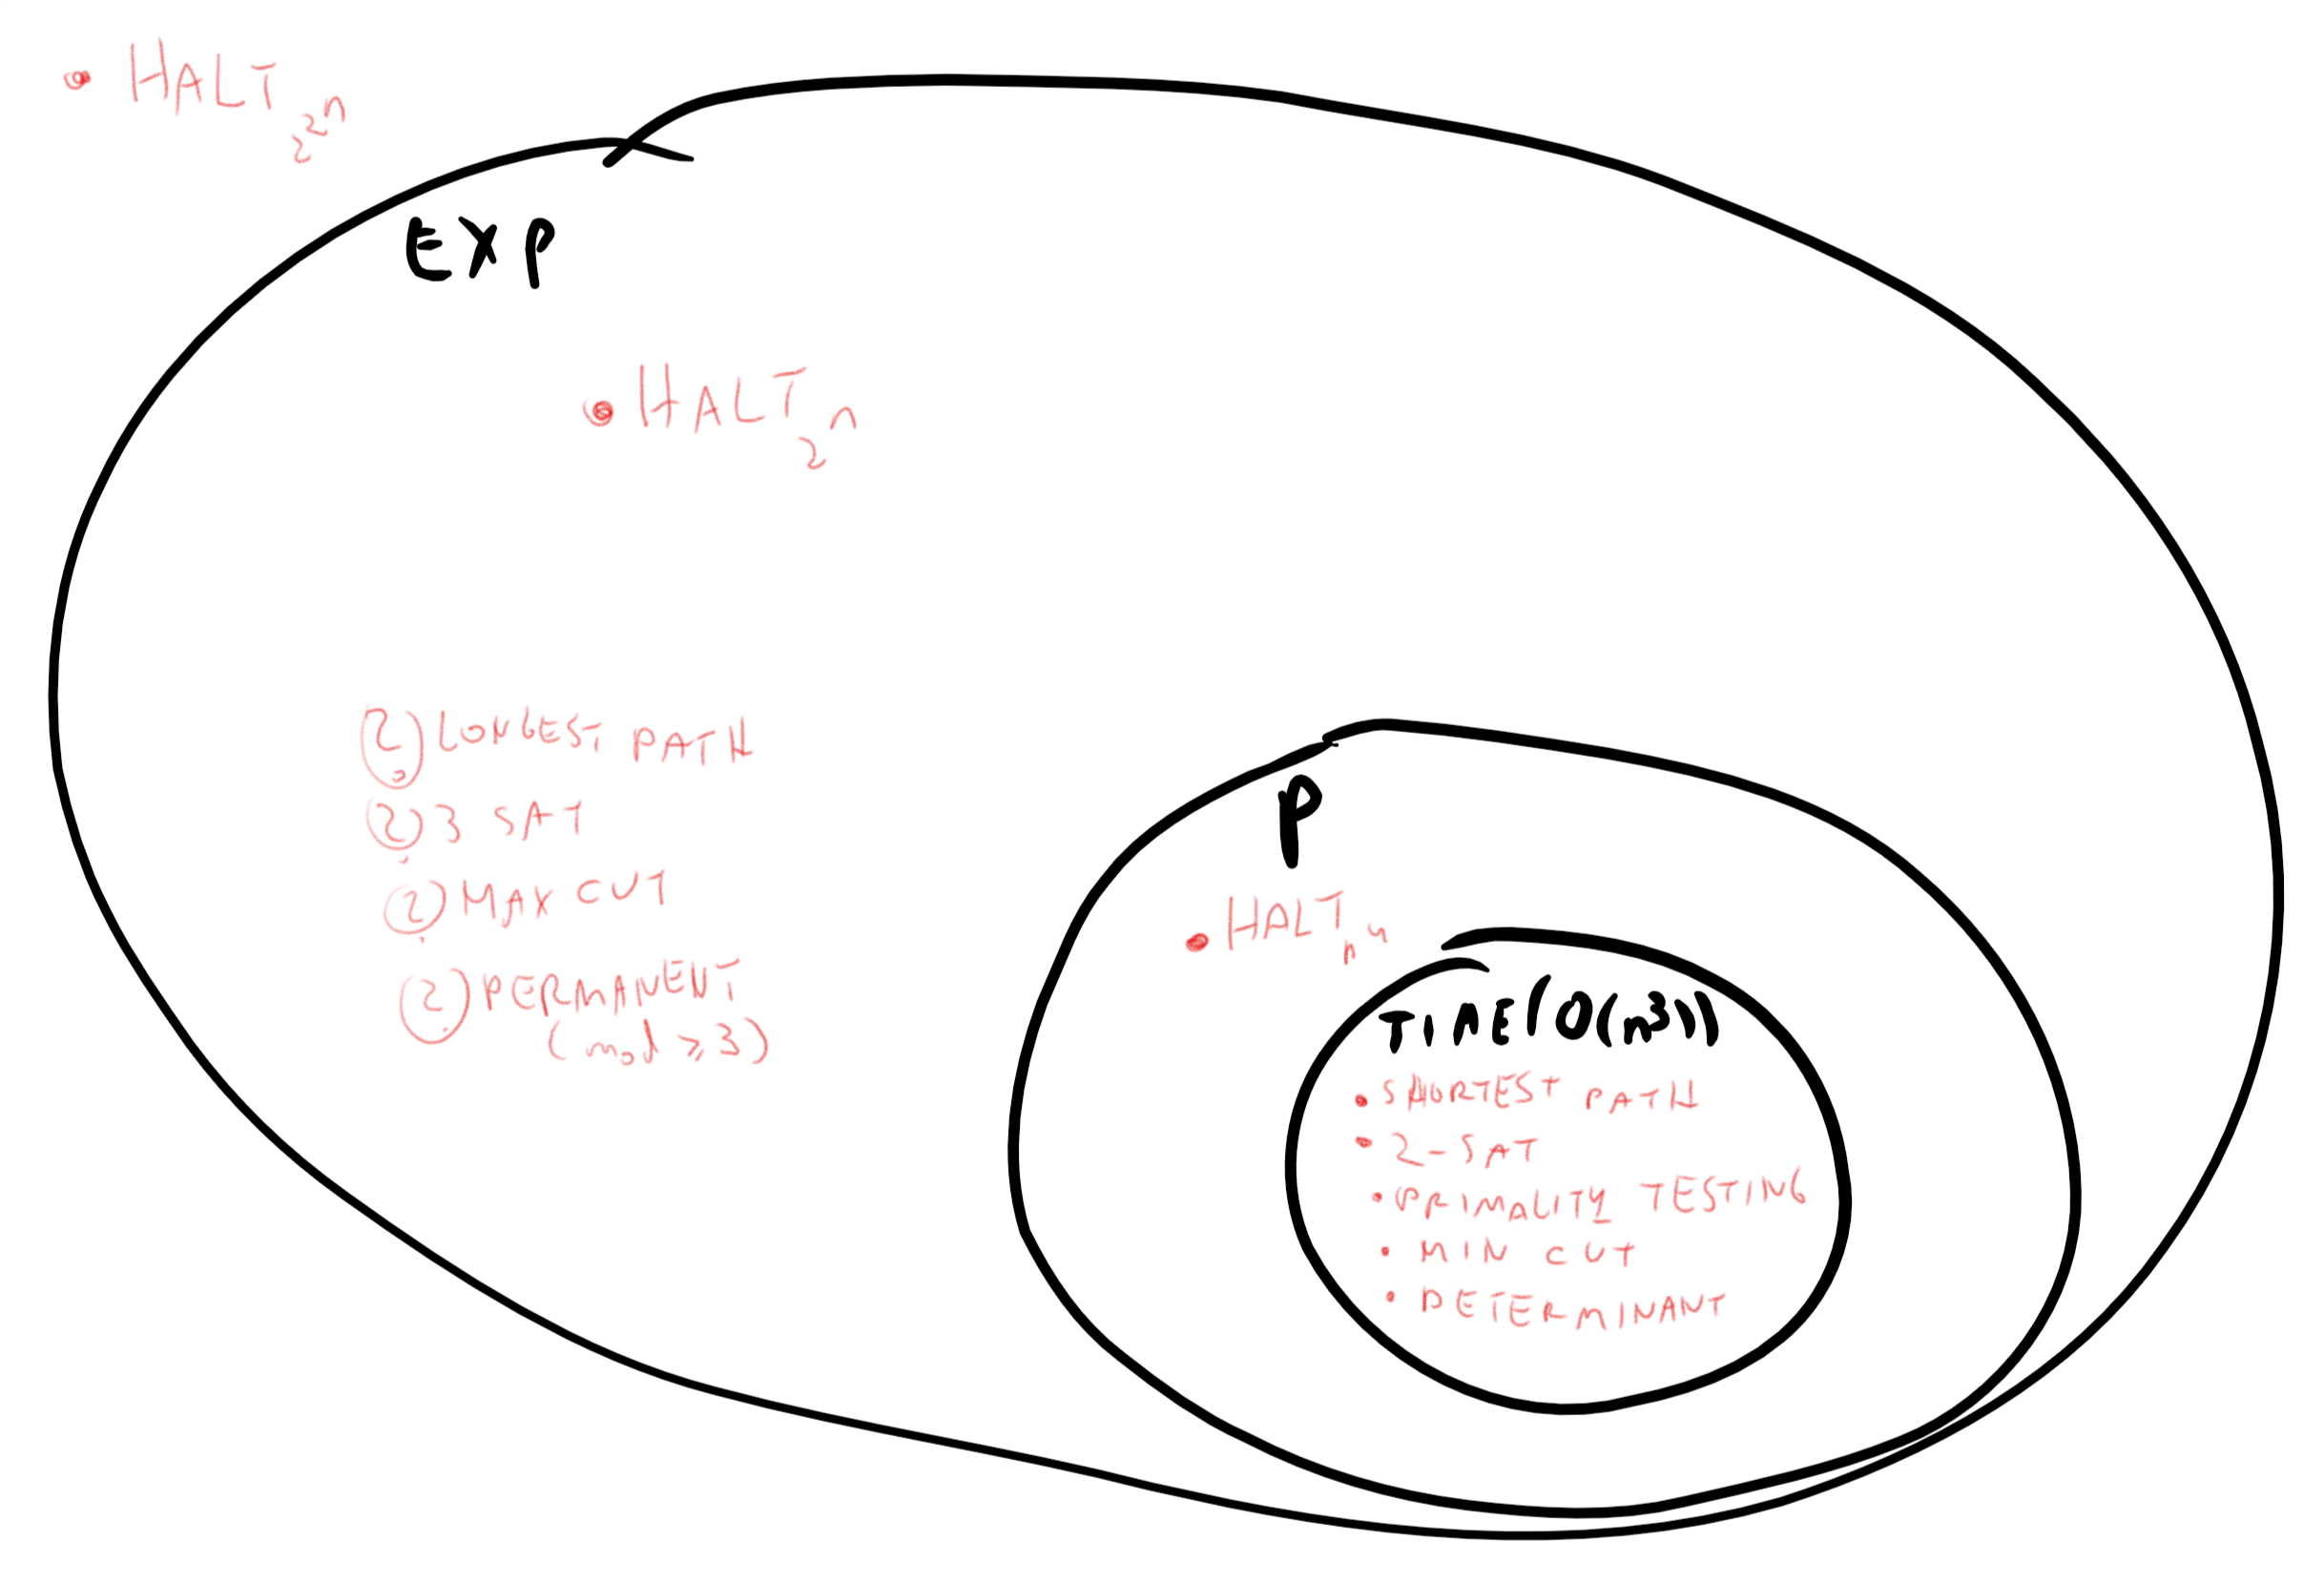
\includegraphics[width=\linewidth, height=1.5in, keepaspectratio]{../figure/time_complexity_map.png}
\caption{Some complexity classes and some of the functions we know (or
conjecture) to be contained in them.}
\label{complexityclassinclusionfig}
\end{marginfigure}

The time hierarchy theorem relies on the existence of an efficient
universal NAND-RAM program, as proven in \cref{univ-nandpp}. For other
models such as Turing Machines we have similar time hierarchy results
showing that there are functions computable in time \(T(n)\) and not in
time \(T(n)/f(n)\) where \(f(n)\) corresponds to the overhead in the
corresponding universal machine.

\section{Non uniform computation}\label{nonuniformcompsec}

We have now seen two measures of ``computation cost'' for functions. In
\cref{secdefinesizeclasses} we defined the complexity of computing
\emph{finite} functions using circuits / straightline programs.
Specifically, for a finite function \(g:\{0,1\}^n \rightarrow \{0,1\}\)
and number \(T\in \N\), \(g\in \ensuremath{\mathit{SIZE}}(T)\) if there
is a circuit of at most \(T\) NAND gates (or equivalently a \(T\)-line
NAND-CIRC program) that computes \(g\). To relate this to the classes
\(\ensuremath{\mathit{TIME}}(T(n))\) defined in this chapter we first
need to extend the class \(\ensuremath{\mathit{SIZE}}(T(n))\) from
finite functions to functions with unbounded input length.

\hypertarget{nonuniformdef}{}
\begin{definition}[Non uniform computation] \label[definition]{nonuniformdef}

Let \(F:\{0,1\}^* \rightarrow \{0,1\}\) and \(T:\N \rightarrow \N\) be a
nice time bound. For every \(n\in \N\), define
\(F_{\upharpoonright n} : \{0,1\}^n \rightarrow \{0,1\}\) to be the
\emph{restriction} of \(F\) to inputs of size \(n\). That is,
\(F_{\upharpoonright n}\) is the function mapping \(\{0,1\}^n\) to
\(\{0,1\}\) such that for every \(x\in \{0,1\}^n\),
\(F_{\upharpoonright n}(x)=F(x)\).

We say that \(F\) is \emph{non-uniformly computable in at most \(T(n)\)
size}, denoted by \(F \in \ensuremath{\mathit{SIZE}}(T(n))\) if there
exists a sequence \((C_0,C_1,C_2,\ldots)\) of NAND circuits such that:

\begin{itemize}
\item
  For every \(n\in \N\), \(C_n\) computes the function
  \(F_{\upharpoonright n}\)
\item
  For every sufficiently large \(n\), \(C_n\) has at most \(T(n)\)
  gates.
\end{itemize}

\end{definition}

The non uniform analog to the class \(\mathbf{P}\) is the class
\(\mathbf{P_{/poly}}\) defined as

\[
\mathbf{P_{/poly}} = \cup_{c\in \N} \ensuremath{\mathit{SIZE}}(n^c)  \; . \label{eqppolydef}
\] There is a big difference between non uniform computation and uniform
complexity classes such as \(\ensuremath{\mathit{TIME}}(T(n))\) or
\(\mathbf{P}\). The condition \(F\in \mathbf{P}\) means that there is a
\emph{single} Turing machine \(M\) that computes \(F\) on all inputs in
polynomial time. The condition \(F\in \mathbf{P_{/poly}}\) only means
that for every input length \(n\) there can be a \emph{different}
circuit \(C_n\) that computes \(F\) using polynomially many gates on
inputs of these lengths. As we will see, \(F\in \mathbf{P_{/poly}}\)
does not necessarily imply that \(F\in \mathbf{P}\). However, the other
direction is true:


\begin{marginfigure}
\centering
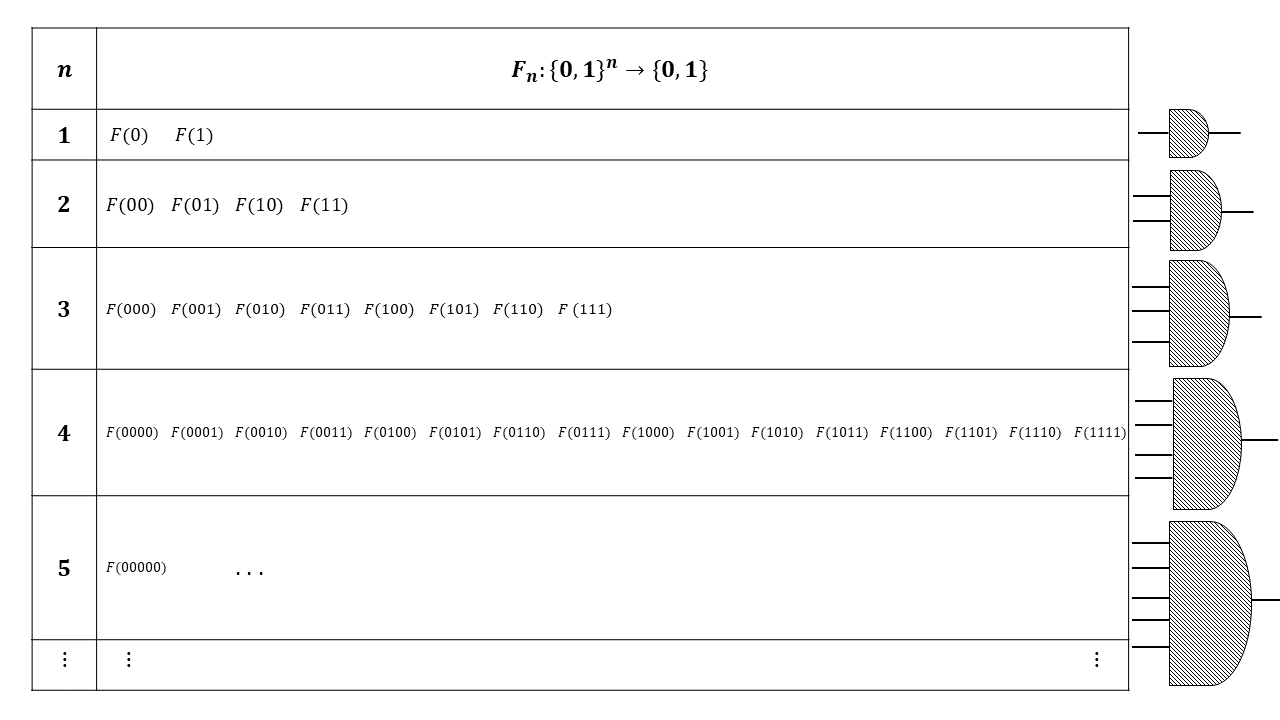
\includegraphics[width=\linewidth, height=1.5in, keepaspectratio]{../figure/Ppoly.png}
\caption{We can think of an infinite function
\(F:\{0,1\}^* \rightarrow \{0,1\}\) as a collection of finite functions
\(F_0,F_1,F_2,\ldots\) where
\(F_{\upharpoonright n}:\{0,1\}^n \rightarrow \{0,1\}\) is the
restriction of \(F\) to inputs of length \(n\). We say \(F\) is in
\(\mathbf{P_{/poly}}\) if for every \(n\), the function
\(F_{\upharpoonright n}\) is computable by a polynomial size NAND-CIRC
program, or equivalently, a polynomial sized Boolean circuit.}
\label{Ppolyfig}
\end{marginfigure}

\hypertarget{non-uniform-thm}{}
\begin{theorem}[Nonuniform computation contains uniform computation] \label[theorem]{non-uniform-thm}

There is some \(a\in \N\) s.t. for every nice \(T:\N \rightarrow \N\)
and \(F:\{0,1\}^* \rightarrow \{0,1\}\),
\[\ensuremath{\mathit{TIME}}(T(n)) \subseteq \ensuremath{\mathit{SIZE}}(T(n)^a)\;.\]

\end{theorem}

In particular, \cref{non-uniform-thm} shows that for every \(c\),
\(\ensuremath{\mathit{TIME}}(n^c) \subseteq \ensuremath{\mathit{SIZE}}(n^{ca})\)
and hence \(\mathbf{P} \subseteq \mathbf{P_{/poly}}\).

\begin{proofidea} \label[proofidea]{The-idea-behind-the-proof}

The idea behind the proof is to ``unroll the loop''. Specifically, we
will use the programming language variants of non-uniform and uniform
computation: namely NAND-CIRC and NAND-TM. The main difference between
the two is that NAND-TM has \emph{loops}. However, for every fixed
\(n\), if we know that a NAND-TM program runs in at most \(T(n)\) steps,
then we can replace its loop by simply ``copying and pasting'' its code
\(T(n)\) times, similar to how in Python we can replace code such as

\begin{code}
for i in range(4):
    print(i)
\end{code}

with the ``loop free'' code

\begin{code}
print(0)
print(1)
print(2)
print(3)
\end{code}

To make this idea into an actual proof we need to tackle one technical
difficulty, and this is to ensure that the NAND-TM program is
\emph{oblivious} in the sense that the value of the index variable
\texttt{i} in the \(j\)-th iteration of the loop will depend only on
\(j\) and not on the contents of the input. We make a digression to do
just that in \cref{obliviousnandtm} and then complete the proof of
\cref{non-uniform-thm}.

\end{proofidea}

\subsection{Oblivious NAND-TM programs}\label{obliviousnandtm}

Our approach for proving \cref{non-uniform-thm} involves ``unrolling the
loop''. For example, consider the following NAND-TM to compute the
\(\ensuremath{\mathit{XOR}}\) function on inputs of arbitrary length:

\begin{code}
temp_0 = NAND(X[0],X[0])
Y_nonblank[0] = NAND(X[0],temp_0)
temp_2 = NAND(X[i],Y[0])
temp_3 = NAND(X[i],temp_2)
temp_4 = NAND(Y[0],temp_2)
Y[0] = NAND(temp_3,temp_4)
MODANDJUMP(X_nonblank[i],X_nonblank[i])
\end{code}

Setting (as an example) \(n=3\), we can attempt to translate this
NAND-TM program into a NAND-CIRC program for computing
\(\ensuremath{\mathit{XOR}}_3:\{0,1\}^3 \rightarrow \{0,1\}\) by simply
``copying and pasting'' the loop three times (dropping the
\texttt{MODANDJMP} line):

\begin{code}
temp_0 = NAND(X[0],X[0])
Y_nonblank[0] = NAND(X[0],temp_0)
temp_2 = NAND(X[i],Y[0])
temp_3 = NAND(X[i],temp_2)
temp_4 = NAND(Y[0],temp_2)
Y[0] = NAND(temp_3,temp_4)
temp_0 = NAND(X[0],X[0])
Y_nonblank[0] = NAND(X[0],temp_0)
temp_2 = NAND(X[i],Y[0])
temp_3 = NAND(X[i],temp_2)
temp_4 = NAND(Y[0],temp_2)
Y[0] = NAND(temp_3,temp_4)
temp_0 = NAND(X[0],X[0])
Y_nonblank[0] = NAND(X[0],temp_0)
temp_2 = NAND(X[i],Y[0])
temp_3 = NAND(X[i],temp_2)
temp_4 = NAND(Y[0],temp_2)
Y[0] = NAND(temp_3,temp_4)
\end{code}

However, the above is still not a valid NAND-CIRC program since it
contains references to the special variable \texttt{i}. To make it into
a valid NAND-CIRC program, we replace references to \texttt{i} in the
first iteration with \(0\), references in the second iteration with
\(1\), and references in the third iteration with \(2\). (We also create
a variable \texttt{zero} and use it for the first time any variable is
instantiated, as well as remove assignments to non-output variables that
are never used later on.) The resulting program is a standard ``loop
free and index free'' NAND-CIRC program that computes
\(\ensuremath{\mathit{XOR}}_3\) (see also \cref{unrolledcircuitfig}):

\begin{code}
temp_0 = NAND(X[0],X[0])
one = NAND(X[0],temp_0)
zero = NAND(one,one)
temp_2 = NAND(X[0],zero)
temp_3 = NAND(X[0],temp_2)
temp_4 = NAND(zero,temp_2)
Y[0] = NAND(temp_3,temp_4)
temp_2 = NAND(X[1],Y[0])
temp_3 = NAND(X[1],temp_2)
temp_4 = NAND(Y[0],temp_2)
Y[0] = NAND(temp_3,temp_4)
temp_2 = NAND(X[2],Y[0])
temp_3 = NAND(X[2],temp_2)
temp_4 = NAND(Y[0],temp_2)
Y[0] = NAND(temp_3,temp_4)
\end{code}


\begin{marginfigure}
\centering
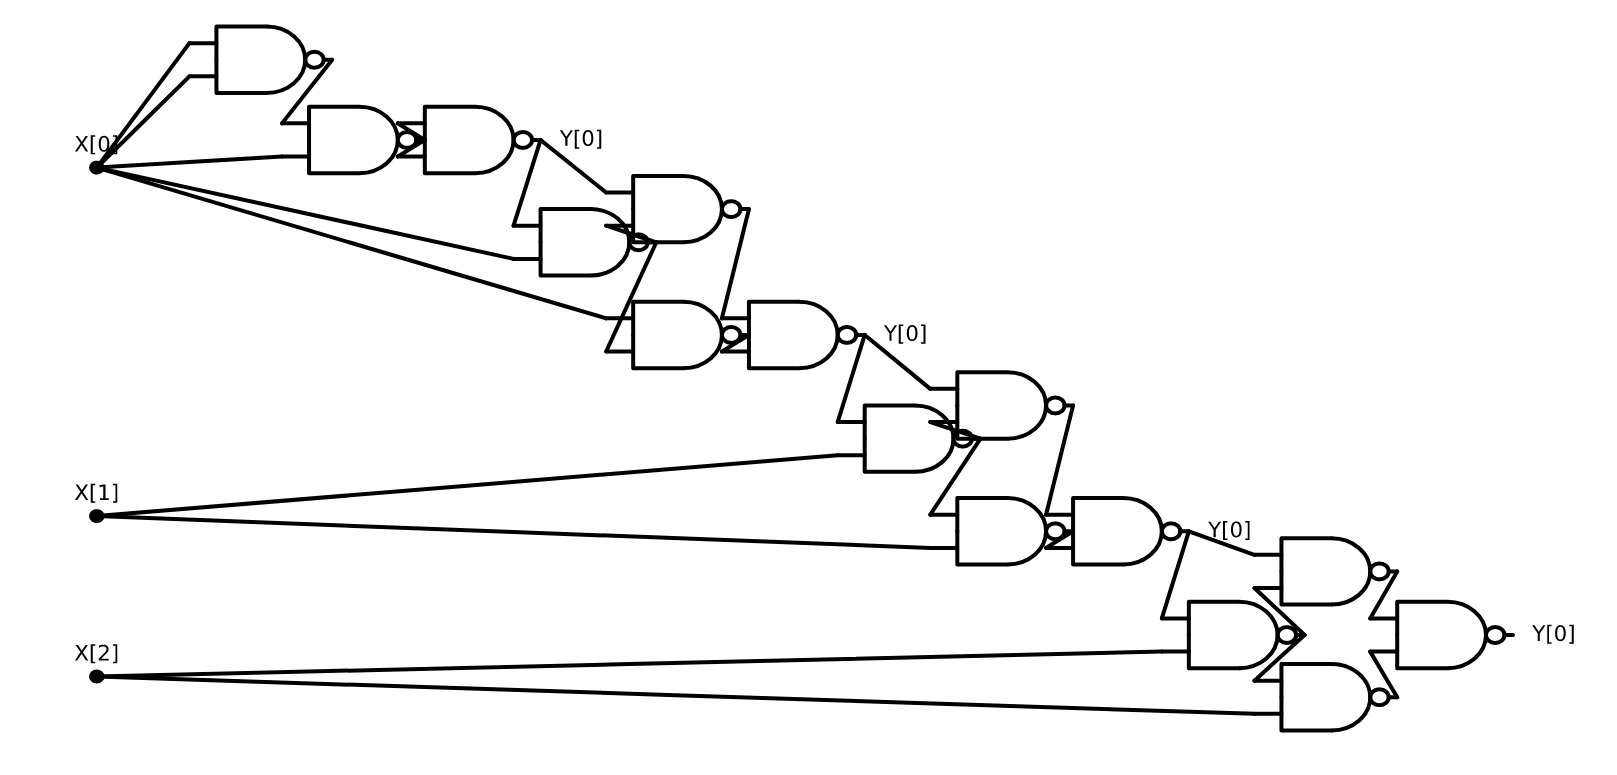
\includegraphics[width=\linewidth, height=1.5in, keepaspectratio]{../figure/unrolled_circuit.png}
\caption{A NAND circuit for \(\ensuremath{\mathit{XOR}}_3\) obtained by
``unrolling the loop'' of the NAND-TM program for computing
\(\ensuremath{\mathit{XOR}}\) three times.}
\label{unrolledcircuitfig}
\end{marginfigure}

Key to this transformation was the fact that in our original NAND-TM
program for \(\ensuremath{\mathit{XOR}}\), regardless of whether the
input is \(011\), \(100\), or any other string, the index variable
\texttt{i} is guaranteed to equal \(0\) in the first iteration, \(1\) in
the second iteration, \(2\) in the third iteration, and so on and so
forth. The particular sequence \(0,1,2,\ldots\) is immaterial: the
crucial property is that the NAND-TM program for
\(\ensuremath{\mathit{XOR}}\) is \emph{oblivious} in the sense that the
value of the index \texttt{i} in the \(j\)-th iteration depends only on
\(j\) and does not depend on the particular choice of the input.
Luckily, it is possible to transform every NAND-TM program into a
functionally equivalent oblivious program with at most quadratic .
(Similarly we can transform any Turing machine into a functionally
equivalent oblivious Turing machine, see \cref{oblivious-ex}.)

\hypertarget{obliviousnandtmthm}{}
\begin{theorem}[Making NAND-TM oblivious] \label[theorem]{obliviousnandtmthm}

Let \(T:\N \rightarrow \N\) be a nice function and let
\(F\in \ensuremath{\mathit{TIME}}_{\mathsf{TM}}(T(n))\). Then there is a
NAND-TM program \(P\) that computes \(F\) in \(O(T(n)^2)\) steps and
satisfying the following. For every \(n\in \N\) there is a sequence
\(i_0,i_1,\ldots, i_{m-1}\) such that for every \(x\in \{0,1\}^n\), if
\(P\) is executed on input \(x\) then in the \(j\)-th iteration the
variable \texttt{i} is equal to \(i_j\).

\end{theorem}

In other words, \cref{obliviousnandtmthm} implies that if we can compute
\(F\) in \(T(n)\) steps, then we can compute it in \(O(T(n)^2)\) steps
with a program \(P\) in which the position of \texttt{i} in the \(j\)-th
iteration depends only on \(j\) and the length of the input, and not on
the contents of the input. Such a program can be easily translated into
a NAND-CIRC program of \(O(T(n)^2)\) lines by ``unrolling the loop''.

\begin{proofidea} \label[proofidea]{We-can-translate-any-NAND}

We can translate any NAND-TM program \(P'\) into an oblivious program
\(P\) by making \(P\) ``sweep'' its arrays. That is, the index
\texttt{i} in \(P\) will always move all the way from position \(0\) to
position \(T(n)-1\) and back again. We can then simulate the program
\(P'\) with at most \(T(n)\) overhead: if \(P'\) wants to move
\texttt{i} left when we are in a rightward sweep then we simply wait the
at most \(2T(n)\) steps until the next time we are back in the same
position while sweeping to the left.

\end{proofidea}


\begin{marginfigure}
\centering
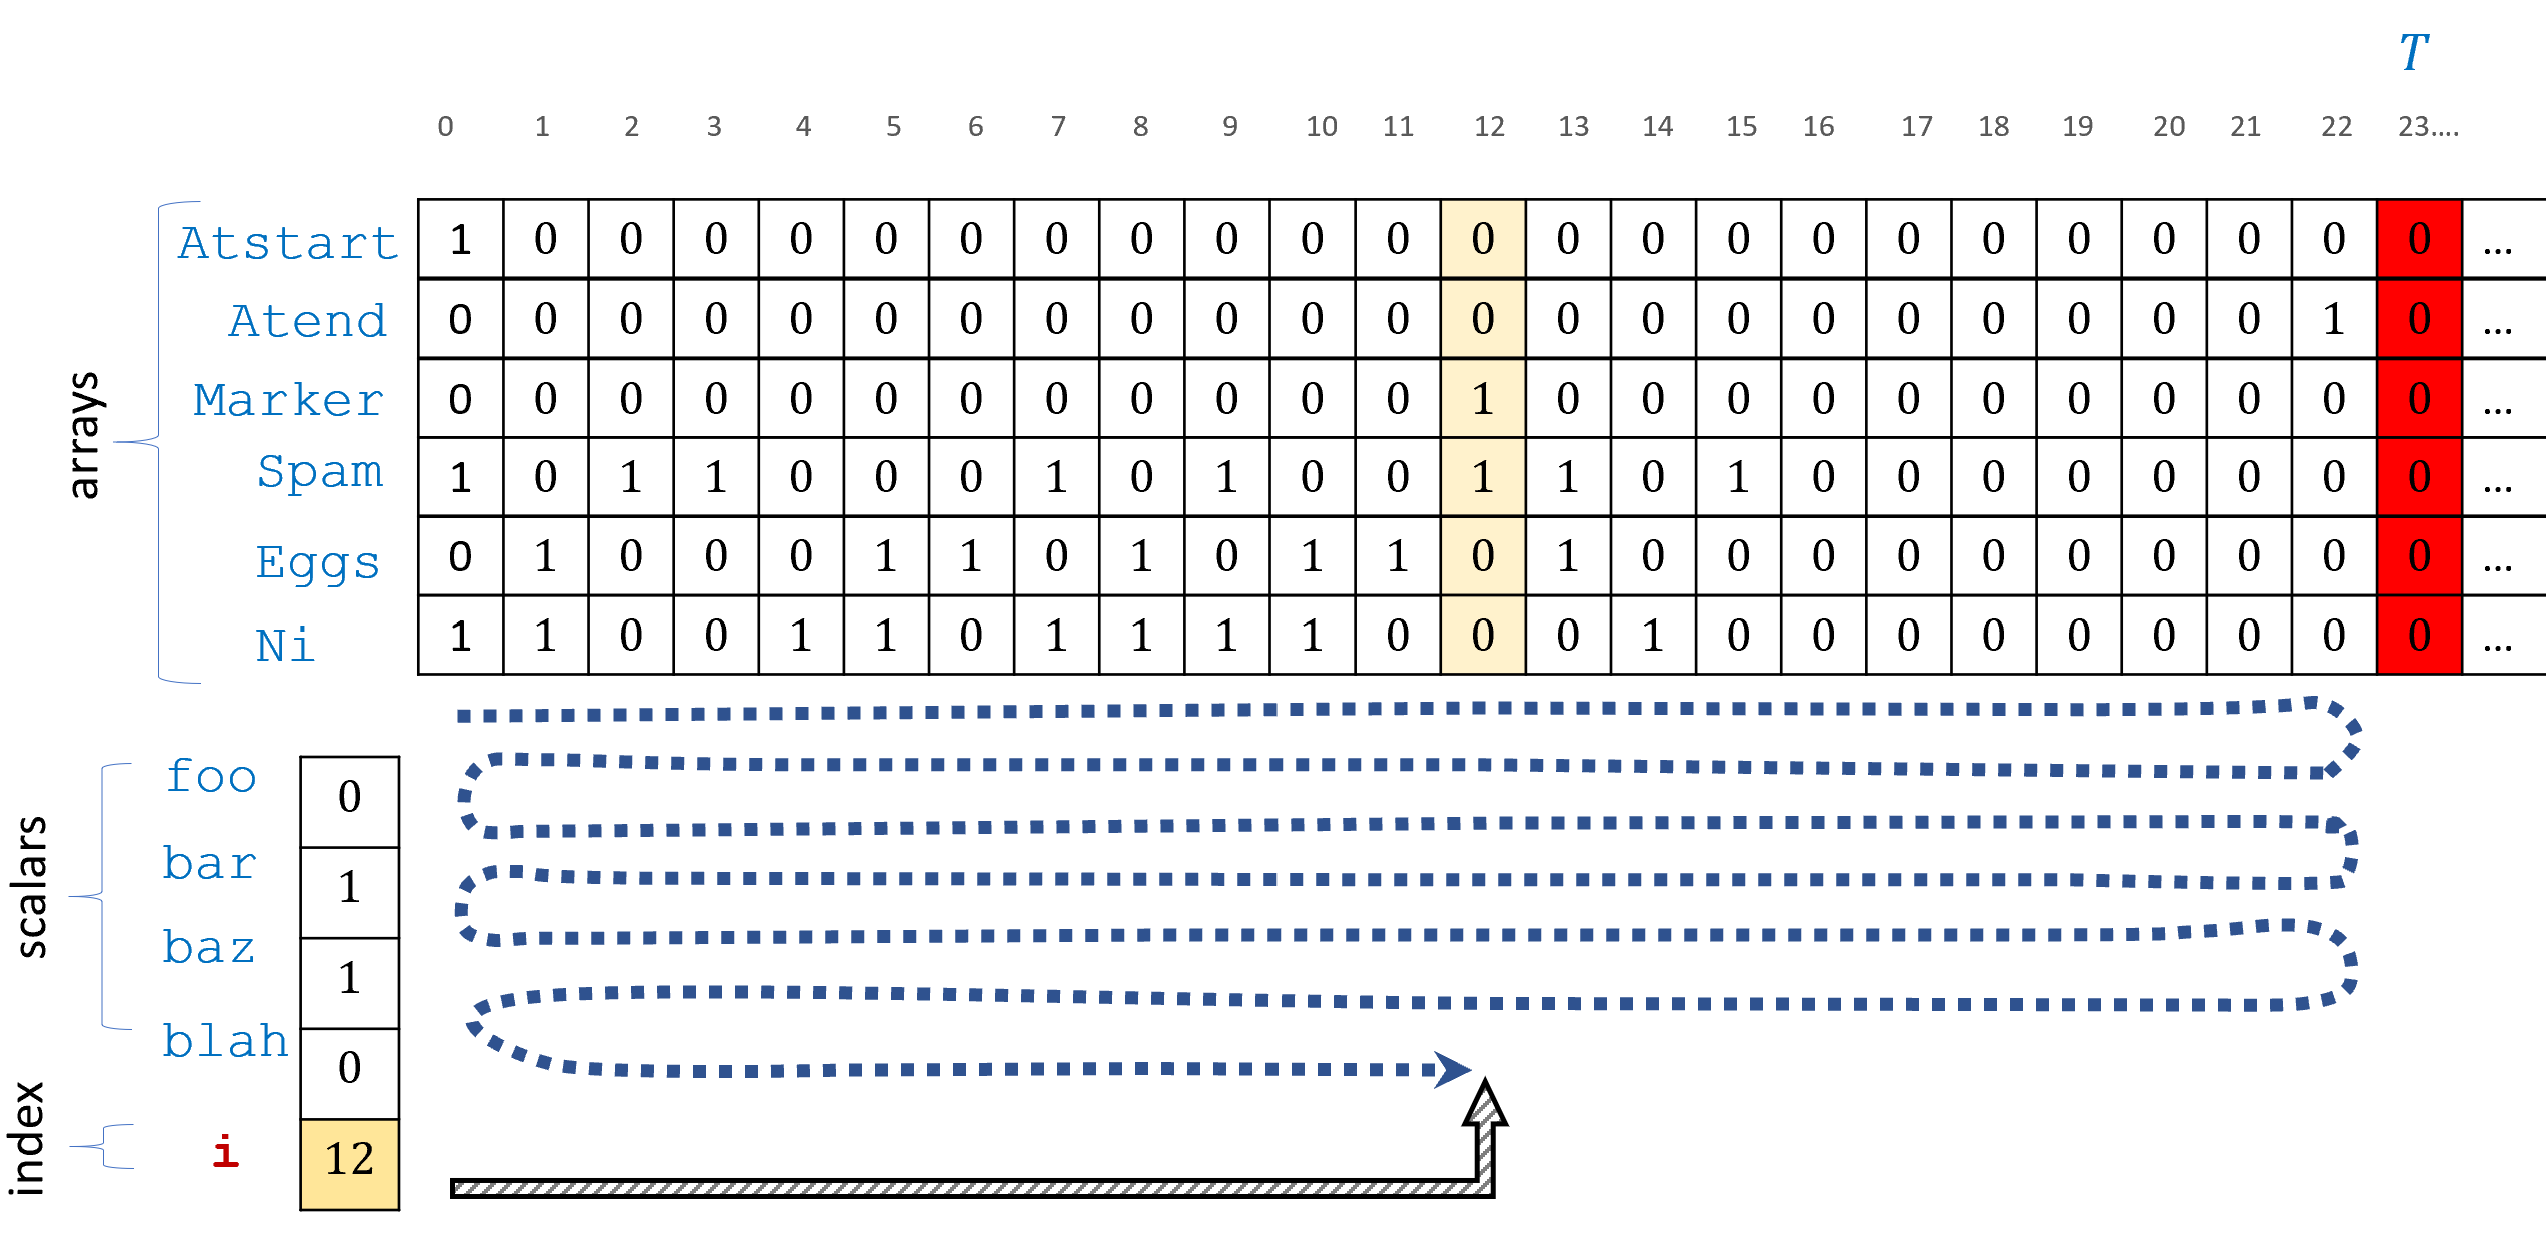
\includegraphics[width=\linewidth, height=1.5in, keepaspectratio]{../figure/obliviousnandtm.png}
\caption{We simulate a \(T(n)\)-time NAND-TM program \(P'\) with an
\emph{oblivious} NAND-TM program \(P\) by adding special arrays
\texttt{Atstart} and \texttt{Atend} to mark positions \(0\) and \(T-1\)
respectively. The program \(P\) will simply ``sweep'' its arrays from
right to left and back again. If the original program \(P'\) would have
moved \texttt{i} in a different direction then we wait \(O(T)\) steps
until we reach the same point back again, and so \(P\) runs in
\(O(T(n)^2)\) time.}
\label{obliviousnandtmfig}
\end{marginfigure}

\begin{proof}[Proof of \cref{obliviousnandtmthm}] \label[proof]{Let-P-be-a-NAND-TM-progra}

Let \(P'\) be a NAND-TM program computing \(F\) in \(T(n)\) steps. We
construct an oblivious NAND-TM program \(P\) for computing \(F\) as
follows (see also \cref{obliviousnandtmfig}).

\begin{enumerate}
\def\labelenumi{\arabic{enumi}.}
\item
  On input \(x\), \(P\) will compute \(T=T(|x|)\) and set up arrays
  \texttt{Atstart} and \texttt{Atend} satisfying
  \texttt{Atstart[}\(0\)\texttt{]}\(=1\) and
  \texttt{Atstart[}\(i\)\texttt{]}\(=0\) for \(i>0\) and
  \texttt{Atend[}\(T-1\)\texttt{]}\(=1\) and
  \texttt{Atend[}i\texttt{]}\(=0\) for all \(i \neq T-1\). We can do
  this because \(T\) is a nice function. Note that since this
  computation does not depend on \(x\) but only on its length, it is
  oblivious.
\item
  \(P\) will also have a special array \texttt{Marker} initialized to
  all zeroes.
\item
  The index variable of \(P\) will change direction of movement to the
  right whenever \texttt{Atstart[i]}\(=1\) and to the left whenever
  \texttt{Atend[i]}\(=1\).
\item
  The program \(P\) simulates the execution of \(P'\). However, if the
  \texttt{MODANDJMP} instruction in \(P'\) attempts to move to the right
  when \(P\) is moving left (or vice versa) then \(P\) will set
  \texttt{Marker[i]} to \(1\) and enter into a special ``waiting mode''.
  In this mode \(P\) will wait until the next time in which
  \texttt{Marker[i]}\(=1\) (at the next sweep) at which points \(P\)
  zeroes \texttt{Marker[i]} and continues with the simulation. In the
  worst case this will take \(2T(n)\) steps (if \(P\) has to go all the
  way from one end to the other and back again.)
\item
  We also modify \(P\) to ensure it ends the computation after
  simulating exactly \(T(n)\) steps of \(P'\), adding ``dummy steps'' if
  \(P'\) ends early.
\end{enumerate}

We see that \(P\) simulates the execution of \(P'\) with an overhead of
\(O(T(n))\) steps of \(P\) per one step of \(P'\), hence completing the
proof.

\end{proof}

\cref{obliviousnandtmthm} implies \cref{non-uniform-thm}. Indeed, if
\(P\) is a \(k\)-line oblivious NAND-TM program computing \(F\) in time
\(T(n)\) then for every \(n\) we can obtain a NAND-CIRC program of
\((k-1)\cdot T(n)\) lines by simply making \(T(n)\) copies of \(P\)
(dropping the final \texttt{MODANDJMP} line). In the \(j\)-th copy we
replace all references of the form \texttt{Foo[i]} to
\texttt{foo\_}\(i_j\) where \(i_j\) is the value of \texttt{i} in the
\(j\)-th iteration.

\subsection{``Unrolling the loop'': algorithmic transformation of Turing
Machines to circuits}\label{unrollloopsec}

The proof of \cref{non-uniform-thm} is \emph{algorithmic}, in the sense
that the proof yields a polynomial-time algorithm that given a Turing
Machine \(M\) and parameters \(T\) and \(n\), produces a circuit of
\(O(T^2)\) gates that agrees with \(M\) on all inputs \(x\in \{0,1\}^n\)
(as long as \(M\) runs for less than \(T\) steps these inputs.) We
record this fact in the following theorem, since it will be useful for
us later on:


\begin{marginfigure}
\centering
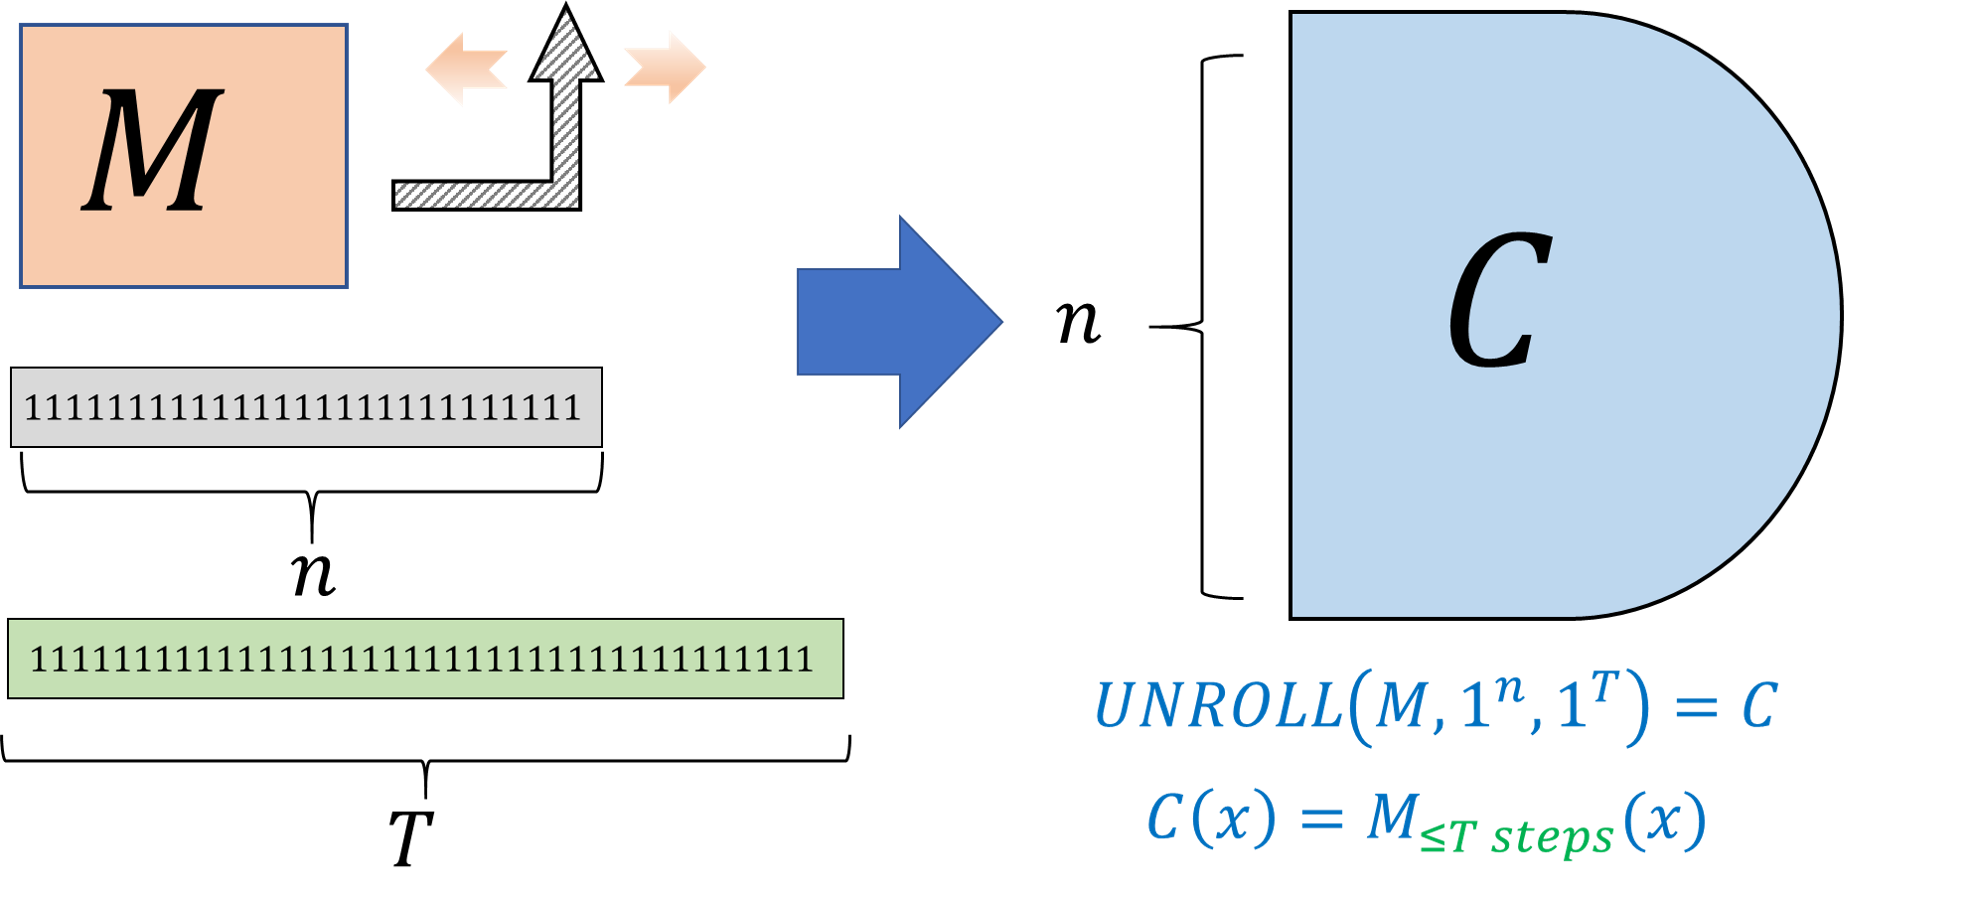
\includegraphics[width=\linewidth, height=1.5in, keepaspectratio]{../figure/unrollloop_alg.png}
\caption{The function \(\ensuremath{\mathit{UNROLL}}\) takes as input a
Turing Machine \(M\), an input length parameter \(n\), a step budget
parameter \(T\), and outputs a circuit \(C\) of size \(poly(T)\) that
takes \(n\) bits of inputs and outputs \(M(x)\) if \(M\) halts on \(x\)
within at most \(T\) steps.}
\label{unrollloopfig}
\end{marginfigure}

\hypertarget{nand-compiler}{}
\begin{theorem}[Turing-machine to circuit compiler] \label[theorem]{nand-compiler}

There is algorithm \(\ensuremath{\mathit{UNROLL}}\) such that for every
Turing Machine \(M\) and numbers \(n,T\),
\(\ensuremath{\mathit{UNROLL}}(M,1^T,1^n)\) runs for \(poly(|M|,T,n)\)
steps and outputs a NAND circuit \(C\) with \(n\) inputs, \(O(T^2)\)
gates, and one output, such that \[
C(x) = \begin{cases}y & M \text{ halts in $\leq T$ steps and outputs $y$} \\ 0 & \text{otherwise} \end{cases}\;.
\]

\end{theorem}

\begin{proof} \label[proof]{We-only-sketch-the-proof-}

We only sketch the proof since it follows by directly translating the
proof of \href{}{non-uniform-thm}\{.ref into an algorithm together with
the simulation of Turing machines by NAND-TM programs (see also
\cref{unrolldescriptionfig}). Specifically,
\(\ensuremath{\mathit{UNROLL}}\) does the following:

\begin{enumerate}
\def\labelenumi{\arabic{enumi}.}
\item
  Transform the Turing Machine \(M\) into an equivalent NAND-TM program
  \(P\).
\item
  Transform the NAND-TM program \(P\) into an equivalent oblivious
  program \(P'\) following the proof of \cref{obliviousnandtmthm}. The
  program \(P'\) takes \(T' = O(T^2)\) steps to simulate \(T\) steps of
  \(P\).
\item
  ``Unroll the loop'' of \(P'\) by obtaining a NAND-CIRC program of
  \(O(T')\) lines (or equivalently a NAND circuit with \(O(T^2)\) gates)
  corresponding to the execution of \(T'\) iterations of \(P'\).
\end{enumerate}

\end{proof}


\begin{figure}
\centering
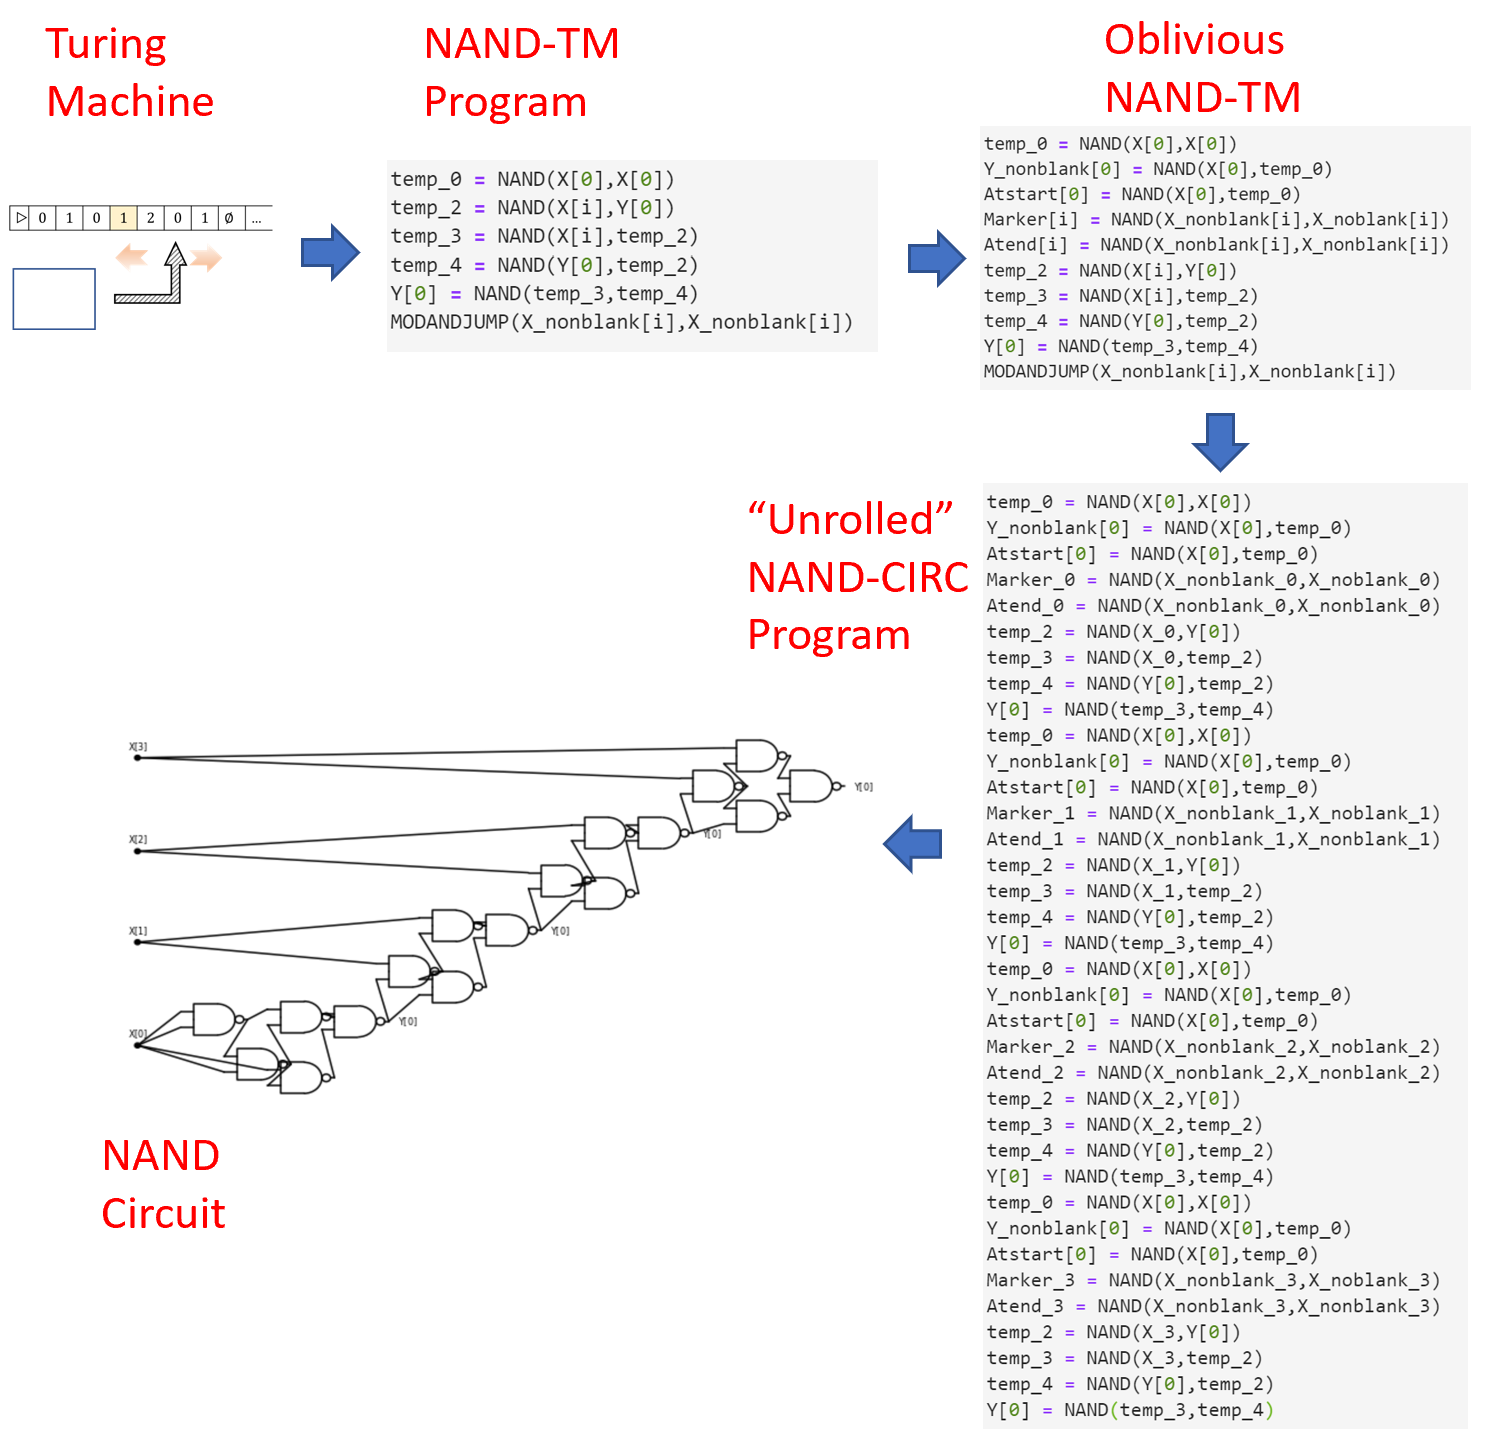
\includegraphics[width=\textwidth, height=0.25\paperheight, keepaspectratio]{../figure/unrolldescription.png}
\caption{We can transform a Turing Machine \(M\), input length parameter
\(n\), and time bound \(T\) into an \(O(T^2)\) sized NAND circuit that
agrees with \(M\) on all inputs \(x\in \{0,1\}^n\) on which \(M\) halts
in at most \(T\) steps. The transformation is obtained by first using
the equivalence of Turing Machines and NAND-TM programs \(P\), then
turning \(P\) into an equivalent \emph{oblivious} NAND-TM program \(P'\)
via \cref{obliviousnandtmthm}, then ``unrolling'' \(O(T^2)\) iterations
of the loop of \(P'\) to obtain an \(O(T^2)\) line NAND-CIRC program
that agrees with \(P'\) on length \(n\) inputs, and finally translating
this program into an equivalent circuit.}
\label{unrolldescriptionfig}
\end{figure}

\hypertarget{unrollloop}{}
\begin{bigidea} \label[bigidea]{unrollloop}

By ``unrolling the loop'' we can transform an algorithm that takes
\(T(n)\) steps to compute \(F\) into a circuit that uses \(poly(T(n))\)
gates to compute the restriction of \(F\) to \(\{0,1\}^n\).

\end{bigidea}

\begin{pause} \label[pause]{Reviewing-the-transformat}

Reviewing the transformations described in \cref{unrolldescriptionfig},
as well as solving the following two exercises is a great way to get
more comfort with non-uniform complexity and in particular with
\(\mathbf{P_{/poly}}\) and its relation to \(\mathbf{P}\).

\end{pause}

\hypertarget{characterizationofp}{}
\begin{solvedexercise}[Alternative characterization of $\mathbf{P}$] \label[solvedexercise]{characterizationofp}

Prove that for every \(F:\{0,1\}^* \rightarrow \{0,1\}\),
\(F\in \mathbf{P}\) if and only if there is a polynomial-time Turing
Machine \(M\) such that for every \(n\in \N\), \(M(1^n)\) outputs a
description of an \(n\) input circuit \(C_n\) that computes the
restriction \(F_{\upharpoonright n}\) of \(F\) to inputs in
\(\{0,1\}^n\).

\end{solvedexercise}

\begin{solution} \label[solution]{We-start-with-the-if-dire}

We start with the ``if'' direction. Suppose that there is a
polynomial-time Turing Machine \(M\) that on input \(1^n\) outputs a
circuit \(C_n\) that computes \(F_{\upharpoonright n}\). Then the
following is a polynomial-time Turing Machine \(M'\) to compute \(F\).
On input \(x\in \{0,1\}^*\), \(M'\) will:

\begin{enumerate}
\def\labelenumi{\arabic{enumi}.}
\item
  Let \(n=|x|\) and compute \(C_n = M(1^n)\).
\item
  Return the evaluation of \(C_n\) on \(x\).
\end{enumerate}

Since we can evaluate a Boolean circuit on an input in polynomial time,
\(M'\) runs in polynomial time and computes \(F(x)\) on every input
\(x\).

For the ``only if'' direction, if \(M'\) is a Turing Machine that
computes \(F\) in polynomial-time, then (applying the equivalence of
Turing Machines and NAND-TM as well as \cref{obliviousnandtmthm}) there
is also an oblivious NAND-TM program \(P\) that computes \(F\) in time
\(p(n)\) for some polynomial \(p\). We can now define \(M\) to be the
Turing Machine that on input \(1^n\) outputs the NAND circuit obtained
by ``unrolling the loop'' of \(P\) for \(p(n)\) iterations. The
resulting NAND circuit computes \(F_{\upharpoonright n}\) and has
\(O(p(n))\) gates. It can also be transformed to a Boolean circuit with
\(O(p(n))\) AND/OR/NOT gates.

\end{solution}

\hypertarget{adviceppoly}{}
\begin{solvedexercise}[$\mathbf{P_{/poly}}$ characterization by advice] \label[solvedexercise]{adviceppoly}

Let \(F:\{0,1\}^* \rightarrow \{0,1\}\). Then \(F\in\mathbf{P_{/poly}}\)
if and only if there exists a polynomial \(p:\N \rightarrow \N\), a
polynomial-time Turing Machine \(M\) and a sequence
\(\{ a_n \}_{n\in \N}\) of strings, such that for every \(n\in \N\):

\begin{itemize}
\tightlist
\item
  \(|a_n| \leq p(n)\)\\
\item
  For every \(x\in \{0,1\}^n\), \(M(a_n,x)=F(x)\).
\end{itemize}

\end{solvedexercise}

\begin{solution} \label[solution]{We-only-sketch-the-proof-}

We only sketch the proof. For the ``only if'' direction, if
\(F\in \mathbf{P_{/poly}}\) then we can use for \(a_n\) simply the
description of the corresponding circuit \(C_n\) and for \(M\) the
program that computes in polynomial time the evaluation of a circuit on
its input.

For the ``if'' direction, we can use the same ``unrolling the loop''
technique of \cref{non-uniform-thm} to show that if \(P\) is a
polynomial-time NAND-TM program, then for every \(n\in \N\), the map
\(x \mapsto P(a_n,x)\) can be computed by a polynomial size NAND-CIRC
program \(Q_n\).

\end{solution}

\subsection{Can uniform algorithms simulate non uniform
ones?}\label{Can-uniform-algorithms-si}

\cref{non-uniform-thm} shows that every function in
\(\ensuremath{\mathit{TIME}}(T(n))\) is in
\(\ensuremath{\mathit{SIZE}}(poly(T(n)))\). One can ask if there is an
inverse relation. Suppose that \(F\) is such that
\(F_{\upharpoonright n}\) has a ``short'' NAND-CIRC program for every
\(n\). Can we say that it must be in
\(\ensuremath{\mathit{TIME}}(T(n))\) for some ``small'' \(T\)? The
answer is an emphatic \textbf{no}. Not only is \(\mathbf{P_{/poly}}\)
not contained in \(\mathbf{P}\), in fact \(\mathbf{P_{/poly}}\) contains
functions that are \emph{uncomputable}!

\hypertarget{Ppolyuncomputable}{}
\begin{theorem}[$\mathbf{P_{/poly}}$ contains uncomputable functions] \label[theorem]{Ppolyuncomputable}

There exists an \emph{uncomputable} function
\(F:\{0,1\}^* \rightarrow \{0,1\}\) such that
\(F \in \mathbf{P_{/poly}}\).

\end{theorem}

\begin{proofidea} \label[proofidea]{Since-mathbfPpoly-corresp}

Since \(\mathbf{P_{/poly}}\) corresponds to non uniform computation, a
function \(F\) is in \(\mathbf{P_{/poly}}\) if for every \(n\in \N\),
the restriction \(F_{\upharpoonright n}\) to inputs of length \(n\) has
a small circuit/program, even if the circuits for different values of
\(n\) are completely different from one another. In particular, if \(F\)
has the property that for every equal-length inputs \(x\) and \(x'\),
\(F(x)=F(x')\) then this means that \(F_{\upharpoonright n}\) is either
the constant function zero or the constant function one for every
\(n\in \N\). Since the constant function has a (very!) small circuit,
such a function \(F\) will always be in \(\mathbf{P_{/poly}}\) (indeed
even in smaller classes). Yet by a reduction from the Halting problem,
we can obtain a function with this property that is uncomputable.

\end{proofidea}

\begin{proof}[Proof of \cref{Ppolyuncomputable}] \label[proof]{Consider-the-following-un}

Consider the following ``unary halting function''
\(\ensuremath{\mathit{UH}}:\{0,1\}^* \rightarrow \{0,1\}\) defined as
follows. We let \(S:\N \rightarrow \{0,1\}^*\) be the function that on
input \(n\in \N\), outputs the string that corresponds to the binary
representation of the number \(n\) without the most significant \(1\)
digit. Note that \(S\) is \emph{onto}. For every \(x\in \{0,1\}\), we
define
\(\ensuremath{\mathit{UH}}(x)=\ensuremath{\mathit{HALTONZERO}}(S(|x|))\).
That is, if \(n\) is the length of \(x\), then
\(\ensuremath{\mathit{UH}}(x)=1\) if and only if the string \(S(n)\)
encodes a NAND-TM program that halts on the input \(0\).

\(\ensuremath{\mathit{UH}}\) is uncomputable, since otherwise we could
compute \(\ensuremath{\mathit{HALTONZERO}}\) by transforming the input
program \(P\) into the integer \(n\) such that \(P=S(n)\) and then
running \(\ensuremath{\mathit{UH}}(1^n)\) (i.e.,
\(\ensuremath{\mathit{UH}}\) on the string of \(n\) ones). On the other
hand, for every \(n\), \(\ensuremath{\mathit{UH}}_n(x)\) is either equal
to \(0\) for all inputs \(x\) or equal to \(1\) on all inputs \(x\), and
hence can be computed by a NAND-CIRC program of a \emph{constant} number
of lines.

\end{proof}

The issue here is of course \emph{uniformity}. For a function
\(F:\{0,1\}^* \rightarrow \{0,1\}\), if \(F\) is in
\(\ensuremath{\mathit{TIME}}(T(n))\) then we have a \emph{single}
algorithm that can compute \(F_{\upharpoonright n}\) for every \(n\). On
the other hand, \(F_{\upharpoonright n}\) might be in
\(\ensuremath{\mathit{SIZE}}(T(n))\) for every \(n\) using a completely
different algorithm for every input length. For this reason we typically
use \(\mathbf{P_{/poly}}\) not as a model of \emph{efficient}
computation but rather as a way to model \emph{inefficient computation}.
For example, in cryptography people often define an encryption scheme to
be secure if breaking it for a key of length \(n\) requires more than a
polynomial number of NAND lines. Since
\(\mathbf{P} \subseteq \mathbf{P_{/poly}}\), this in particular
precludes a polynomial time algorithm for doing so, but there are
technical reasons why working in a non uniform model makes more sense in
cryptography. It also allows to talk about security in non asymptotic
terms such as a scheme having ``\(128\) bits of security''.

While it can sometimes be a real issue, in many natural settings the
difference between uniform and non-uniform computation does not seem to
so important. In particular, in all the examples of problems not known
to be in \(\mathbf{P}\) we discussed before: longest path, 3SAT,
factoring, etc., these problems are also not known to be in
\(\mathbf{P_{/poly}}\) either. Thus, for ``natural'' functions, if you
pretend that \(\ensuremath{\mathit{TIME}}(T(n))\) is roughly the same as
\(\ensuremath{\mathit{SIZE}}(T(n))\), you will be right more often than
wrong.


\begin{figure}
\centering
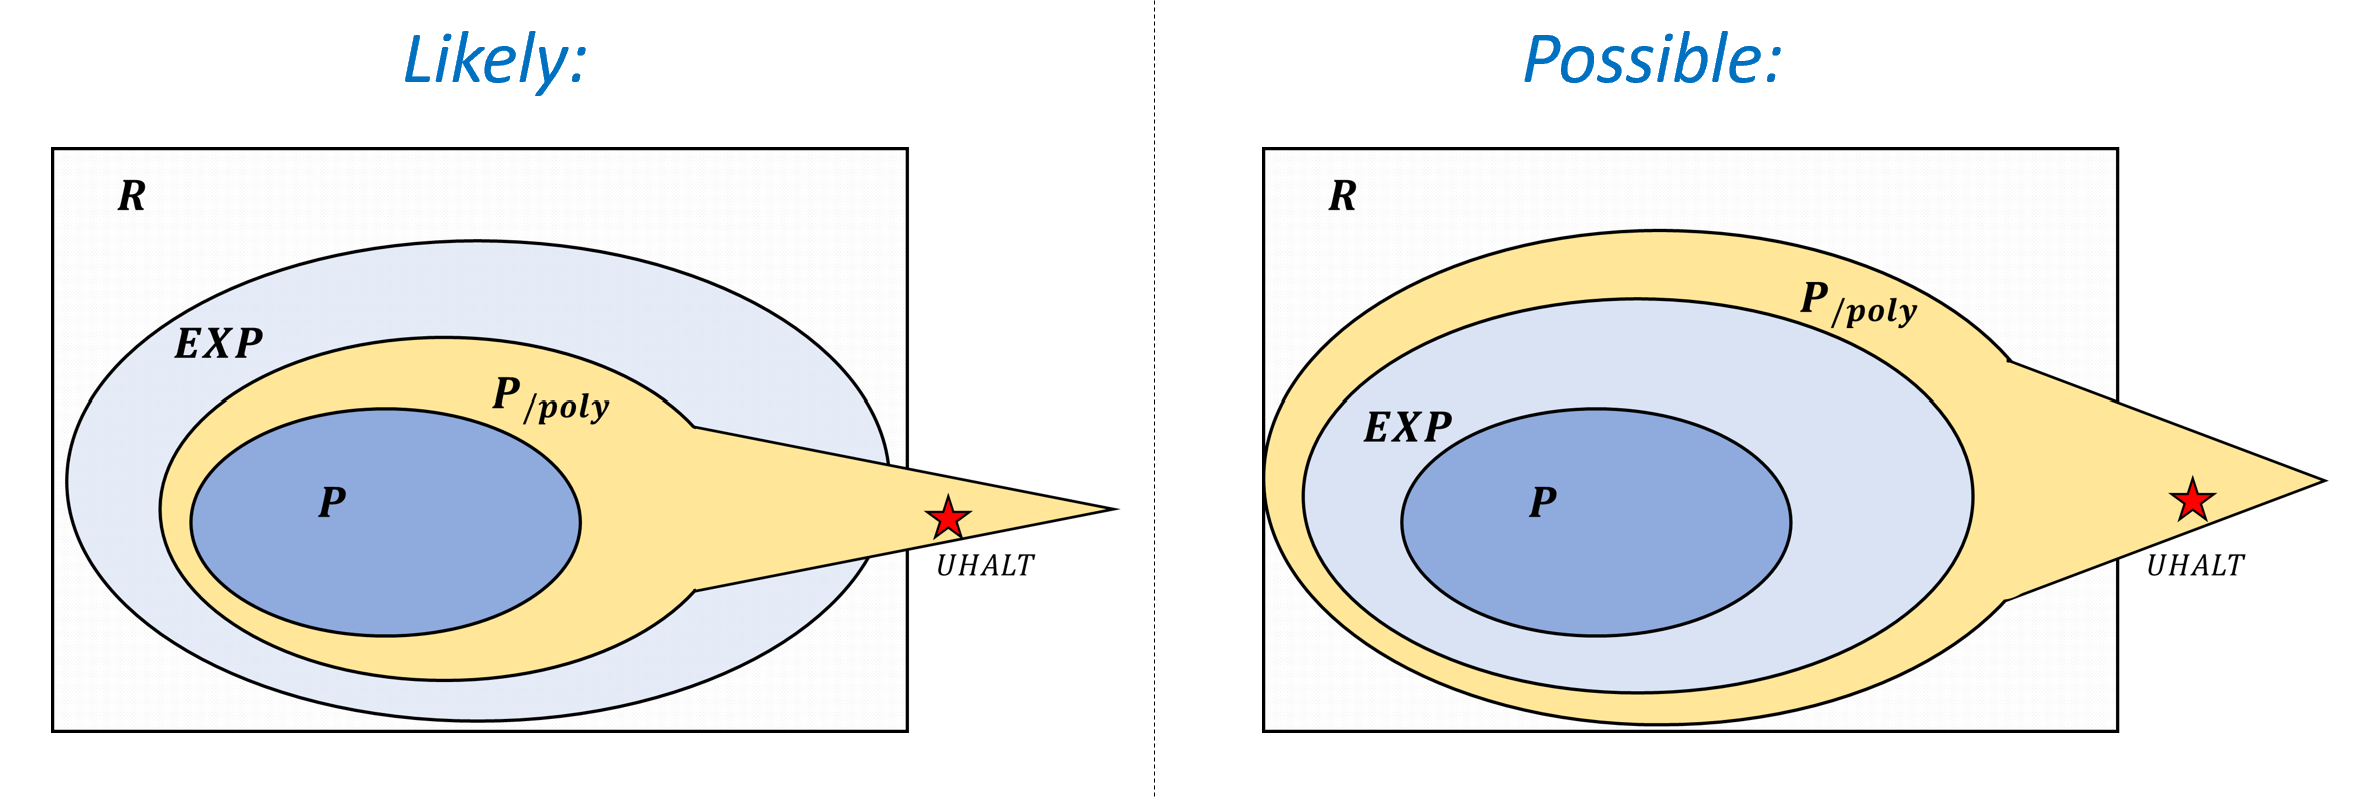
\includegraphics[width=\textwidth, height=0.25\paperheight, keepaspectratio]{../figure/PEXPPpolyrelations.png}
\caption{Relations between \(\mathbf{P}\), \(\mathbf{EXP}\), and
\(\mathbf{P_{/poly}}\). It is known that
\(\mathbf{P} \subseteq \mathbf{EXP}\),
\(\mathbf{P} \subseteq \mathbf{P_{/poly}}\) and that
\(\mathbf{P_{/poly}}\) contains uncomputable functions (which in
particular are outside of \(\mathbf{EXP}\)). It is not known whether or
not \(\mathbf{EXP} \subseteq \mathbf{P_{/poly}}\) though it is believed
that \(\mathbf{EXP} \not\subseteq \mathbf{P_{/poly}}\).}
\label{PEXPPpolyrelationsfig}
\end{figure}

\subsection{Uniform vs.~Nonuniform computation: A
recap}\label{Uniform-vsNonuniform-comp}

To summarize, the two models of computation we have described so far
are:

\begin{itemize}
\item
  \textbf{Uniform models:} \emph{Turing machines}, \emph{NAND-TM
  programs}, \emph{RAM machines}, \emph{NAND-RAM programs},
  \emph{C/JavaScript/Python}, etc. These model include loops and
  unbounded memory hence a single program can compute a function with
  unbounded input length.
\item
  \textbf{Non-uniform models:} \emph{Boolean Circuits} or
  \emph{straightline programs} have no loops and can only compute finite
  functions. The time to execute them is exactly the number of lines or
  gates they contain.
\end{itemize}

For a function \(F:\{0,1\}^* \rightarrow \{0,1\}\) and some nice time
bound \(T:\N \rightarrow \N\), we know that:

\begin{itemize}
\item
  If \(F\) is uniformly computable in time \(T(n)\) then there is a
  sequence of circuits \(C_1,C_2,\ldots\) where \(C_n\) has
  \(poly(T(n))\) gates and computes \(F_{\upharpoonright n}\) (i.e.,
  restriction of \(F\) to \(\{0,1\}^n\)) for every \(n\).
\item
  The reverse direction is not necessarily true - there are examples of
  functions \(F:\{0,1\}^n \rightarrow \{0,1\}\) such that
  \(F_{\upharpoonright n}\) can be computed by even a constant size
  circuit but \(F\) is uncomputable.
\end{itemize}

This means that non uniform complexity is more useful to establish
\emph{hardness} of a function than its \emph{easiness}.

\begin{recap} \label[recap]{We-can-define-the-time-co}

\begin{itemize}
\item
  We can define the time complexity of a function using NAND-TM
  programs, and similarly to the notion of computability, this appears
  to capture the inherent complexity of the function.
\item
  There are many natural problems that have polynomial-time algorithms,
  and other natural problems that we'd love to solve, but for which the
  best known algorithms are exponential.
\item
  The definition of polynomial time, and hence the class \(\mathbf{P}\),
  is robust to the choice of model, whether it is Turing machines,
  NAND-TM, NAND-RAM, modern programming languages, and many other
  models.
\item
  The time hierarchy theorem shows that there are \emph{some} problems
  that can be solved in exponential, but not in polynomial time.
  However, we do not know if that is the case for the natural examples
  that we described in this lecture.
\item
  By ``unrolling the loop'' we can show that every function computable
  in time \(T(n)\) can be computed by a sequence of NAND-CIRC programs
  (one for every input length) each of size at most \(poly(T(n))\)
\end{itemize}

\end{recap}

\section{Exercises}\label{Exercises}

\hypertarget{definitionofP}{}
\begin{exercise}[Equivalence of different definitions of $\mathbf{P}$ and $\mathbf{EXP}$.] \label[exercise]{definitionofP}

Prove that the classes \(\mathbf{P}\) and \(\mathbf{EXP}\) defined in
\cref{PandEXPdef} are equal to
\(\cup_{c\in \{1,2,3,\ldots \}} \ensuremath{\mathit{TIME}}(n^c)\) and
\(\cup_{c\in \{1,2,3,\ldots \}} \ensuremath{\mathit{TIME}}(2^{n^c})\)
respectively. (If \(S_1,S_2,S_3,\ldots\) is a collection of sets then
the set \(S = \cup_{c\in \{1,2,3,\ldots \}} S_c\) is the set of all
elements \(e\) such that there exists some \(c\in \{ 1,2,3,\ldots \}\)
where \(e\in S_c\).)

\end{exercise}

\hypertarget{robsutrepresex}{}
\begin{exercise}[Robustness to representation] \label[exercise]{robsutrepresex}

\cref{polyRAMTM-thm} shows that the classes \(\mathbf{P}\) and
\(\mathbf{EXP}\) are \emph{robust} with respect to variations in the
choice of the computational model. This exercise shows that these
classes are also robust with respect to our choice of the representation
of the input.

Specifically, let \(F\) be a function mapping graphs to \(\{0,1\}\), and
let \(F', F'':\{0,1\}^* \rightarrow \{0,1\}\) be the functions defined
as follows. For every \(x\in \{0,1\}^*\):

\begin{itemize}
\item
  \(F'(x)=1\) iff \(x\) represents a graph \(G\) via the adjacency
  matrix representation such that \(F(G)=1\).
\item
  \(F''(x)=1\) iff \(x\) represents a graph \(G\) via the adjacency list
  representation such that \(F(G)=1\).
\end{itemize}

Prove that \(F' \in \mathbf{P}\) iff \(F'' \in \mathbf{P}\).

More generally, for every function \(F:\{0,1\}^* \rightarrow \{0,1\}\),
the answer to the question of whether \(F\in \mathbf{P}\) (or whether
\(F\in \mathbf{EXP}\)) is unchanged by switching representations, as
long as transforming one representation to the other can be done in
polynomial time (which essentially holds for all reasonable
representations).

\end{exercise}

\hypertarget{boolex}{}
\begin{exercise}[Boolean functions] \label[exercise]{boolex}

For every function \(F:\{0,1\}^* \rightarrow \{0,1\}^*\), define
\(Bool(F)\) to be the function mapping \(\{0,1\}^*\) to \(\{0,1\}\) such
that on input a (string representation of a) triple \((x,i,\sigma)\)
with \(x\in \{0,1\}^*\), \(i \in \N\) and \(\sigma \in \{0,1\}\),

\[
Bool(F)(x,i,\sigma) = \begin{cases} F(x)_i & \sigma =0, i<|F(x)| \\
                                    1      & \sigma = 1,i<|F(x)| \\
                                 0   & \text{otherwise} \end{cases}
\] where \(F(x)_i\) is the \(i\)-th bit of the string \(F(x)\).

Prove that \(F \in \overline{\mathbf{P}}\) if and only if
\(Bool(F) \in \mathbf{P}\).

\end{exercise}

\hypertarget{poly-time-comp-ex}{}
\begin{exercise}[Composition of polynomial time] \label[exercise]{poly-time-comp-ex}

Prove that if \(F,G:\{0,1\}^* \rightarrow \{0,1\}^*\) are in
\(\overline{\mathbf{P}}\) then their \emph{composition} \(F\circ G\),
which is the function \(H\) s.t. \(H(x)=F(G(x))\), is also in
\(\overline{\mathbf{P}}\).

\end{exercise}

\hypertarget{exp-time-comp-ex}{}
\begin{exercise}[Non composition of exponential time] \label[exercise]{exp-time-comp-ex}

Prove that there is some \(F,G:\{0,1\}^* \rightarrow \{0,1\}^*\) s.t.
\(F,G \in \overline{\mathbf{EXP}}\) but \(F\circ G\) is not in
\(\mathbf{EXP}\).

\end{exercise}

\hypertarget{oblivious-ex}{}
\begin{exercise}[Oblivious Turing Machines] \label[exercise]{oblivious-ex}

We say that a Turing machine \(M\) is \emph{oblivious} if there is some
function \(T:\N\times \N \rightarrow \Z\) such that for every input
\(x\) of length \(n\), and \(t\in \N\) it holds that:

\begin{itemize}
\item
  If \(M\) takes more than \(t\) steps to halt on the input \(x\), then
  in the \(t\)-th step \(M\)'s head will be in the position \(T(n,t)\).
  (Note that this position depends only on the \emph{length} of \(x\)
  and not its contents.)
\item
  If \(M\) halts before the \(t\)-th step then \(T(n,t) = -1\).
\end{itemize}

Prove that if \(F\in \mathbf{P}\) then there exists an \emph{oblivious}
Turing machine \(M\) that computes \(F\) in polynomial time. See
footnote for hint.\footnote{\emph{Hint:} This is the Turing Machine
  analog of \cref{obliviousnandtmthm}. We replace one step of the
  original TM \(M'\) computing \(F\) with a ``sweep'' of the obliviouss
  TM \(M\) in which it goes \(T\) steps to the right and then \(T\)
  steps to the left.}

\end{exercise}

\hypertarget{graphedgeex}{}
\begin{exercise} \label[exercise]{graphedgeex}

Let \(\ensuremath{\mathit{EDGE}}:\{0,1\}^* \rightarrow \{0,1\}\) be the
function such that on input a string representing a triple \((L,i,j)\),
where \(L\) is the adjacency list representation of an \(n\) vertex
graph \(G\), and \(i\) and \(j\) are numbers in \([n]\),
\(\ensuremath{\mathit{EDGE}}(L,i,j)=1\) if the edge \(\{i,j \}\) is
present in the graph. \(\ensuremath{\mathit{EDGE}}\) outputs \(0\) on
all other inputs.

\begin{enumerate}
\def\labelenumi{\arabic{enumi}.}
\item
  Prove that \(\ensuremath{\mathit{EDGE}} \in \mathbf{P}\).
\item
  Let
  \(\ensuremath{\mathit{PLANARMATRIX}}:\{0,1\}^* \rightarrow \{0,1\}\)
  be the function that on input an adjacency matrix \(A\) outputs \(1\)
  if and only if the graph represented by \(A\) is \emph{planar} (that
  is, can be drawn on the plane without edges crossing one another). For
  this question, you can use without proof the fact that
  \(\ensuremath{\mathit{PLANARMATRIX}} \in \mathbf{P}\). Prove that
  \(\ensuremath{\mathit{PLANARLIST}} \in \mathbf{P}\) where
  \(\ensuremath{\mathit{PLANARLIST}}:\{0,1\}^* \rightarrow \{0,1\}\) is
  the function that on input an adjacency list \(L\) outputs \(1\) if
  and only if \(L\) represents a planar graph.
\end{enumerate}

\end{exercise}

\hypertarget{evalnandcircuit}{}
\begin{exercise}[Evaluate NAND circuits] \label[exercise]{evalnandcircuit}

Let \(\ensuremath{\mathit{NANDEVAL}}:\{0,1\}^* \rightarrow \{0,1\}\) be
the function such that for every string representing a pair \((Q,x)\)
where \(Q\) is an \(n\)-input \(1\)-output NAND-CIRC (not NAND-TM!)
program and \(x\in \{0,1\}^n\),
\(\ensuremath{\mathit{NANDEVAL}}(Q,x)=Q(x)\). On all other inputs
\(\ensuremath{\mathit{NANDEVAL}}\) outputs \(0\).

Prove that \(\ensuremath{\mathit{NANDEVAL}} \in \mathbf{P}\).

\end{exercise}

\hypertarget{hardfunc}{}
\begin{exercise}[Find hard function] \label[exercise]{hardfunc}

Let \(\ensuremath{\mathit{NANDHARD}}:\{0,1\}^* \rightarrow \{0,1\}\) be
the function such that on input a string representing a pair \((f,s)\)
where

\begin{itemize}
\tightlist
\item
  \(f \in \{0,1\}^{2^n}\) for some \(n\in \mathbb{N}\)
\item
  \(s\in \mathbb{N}\)
\end{itemize}

\(\ensuremath{\mathit{NANDHARD}}(f,s)=1\) if there is no NAND-CIRC
program \(Q\) of at most \(s\) lines that computes the function
\(F:\{0,1\}^n \rightarrow \{0,1\}\) whose truth table is the string
\(f\). That is, \(\ensuremath{\mathit{NANDHARD}}(f,s)=1\) if for every
NAND-CIRC program \(Q\) of at most \(s\) lines, there exists some
\(x\in \{0,1\}^{n}\) such that \(Q(x) \neq f_x\) where \(f_x\) denote
the \(x\)-the coordinate of \(f\), using the binary representation to
identify \(\{0,1\}^n\) with the numbers \(\{0,\ldots,2^n -1 \}\).

\begin{enumerate}
\def\labelenumi{\arabic{enumi}.}
\item
  Prove that \(\ensuremath{\mathit{NANDHARD}} \in \mathbf{EXP}\).
\item
  (Challenge) Prove that there is an algorithm
  \(\ensuremath{\mathit{FINDHARD}}\) such that if \(n\) is sufficiently
  large, then \(\ensuremath{\mathit{FINDHARD}}(1^n)\) runs in time
  \(2^{2^{O(n)}}\) and outputs a string \(f \in \{0,1\}^{2^n}\) that is
  the truth table of a function that is not contained in
  \(\ensuremath{\mathit{SIZE}}(2^n/(1000n))\). (In other words, if \(f\)
  is the string output by \(\ensuremath{\mathit{FINDHARD}}(1^n)\) then
  if we let \(F:\{0,1\}^n \rightarrow \{0,1\}\) be the function such
  that \(F(x)\) outputs the \(x\)-th coordinate of \(f\), then
  \(F\not\in \ensuremath{\mathit{SIZE}}(2^n/(1000n))\).\footnote{\textbf{Hint:}
    Use Item 1, the existence of functions requiring exponentially hard
    NAND programs, and the fact that there are only finitely many
    functions mapping \(\{0,1\}^n\) to \(\{0,1\}\).}
\end{enumerate}

\end{exercise}

\hypertarget{scheduleprogex}{}
\begin{exercise} \label[exercise]{scheduleprogex}

Suppose that you are in charge of scheduling courses in computer science
in University X. In University X, computer science students wake up
late, and have to work on their startups in the afternoon, and take long
weekends with their investors. So you only have two possible slots: you
can schedule a course either Monday-Wednesday 11am-1pm or
Tuesday-Thursday 11am-1pm.

Let \(\ensuremath{\mathit{SCHEDULE}}:\{0,1\}^* \rightarrow \{0,1\}\) be
the function that takes as input a list of courses \(L\) and a list of
\emph{conflicts} \(C\) (i.e., list of pairs of courses that cannot share
the same time slot) and outputs \(1\) if and only if there is a
``conflict free'' scheduling of the courses in \(L\), where no pair in
\(C\) is scheduled in the same time slot.

More precisely, the list \(L\) is a list of strings
\((c_0,\ldots,c_{n-1})\) and the list \(C\) is a list of pairs of the
form \((c_i,c_j)\). \(\ensuremath{\mathit{SCHEDULE}}(L,C)=1\) if and
only if there exists a partition of \(c_0,\ldots,c_{n-1}\) into two
parts so that there is no pair \((c_i,c_j) \in C\) such that both
\(c_i\) and \(c_j\) are in the same part.

Prove that \(\ensuremath{\mathit{SCHEDULE}} \in \mathbf{P}\). As usual,
you do not have to provide the full code to show that this is the case,
and can describe operations as a high level, as well as appeal to any
data structures or other results mentioned in the book or in lecture.
Note that to show that a function \(F\) is in \(\mathbf{P}\) you need to
both \textbf{(1)} present an algorithm \(A\) that computes \(F\) in
polynomial time, \textbf{(2)} \emph{prove} that \(A\) does indeed run in
polynomial time, and does indeed compute the correct answer.

Try to think whether or not your algorithm extends to the case where
there are \emph{three} possible time slots.

\end{exercise}

\section{Bibliographical notes}\label{bibnotesrunningtime}

Because we are interested in the \emph{maximum} number of steps for
inputs of a given length, running-time as we defined it is often known
as \emph{worst case complexity}. The \emph{minimum} number of steps (or
``best case'' complexity) to compute a function on length \(n\) inputs
is typically not a meaningful quantity since essentially every natural
problem will have some trivially easy instances. However, the
\emph{average case complexity} (i.e., complexity on a ``typical'' or
``random'' input) is an interesting concept which we'll return to when
we discuss \emph{cryptography}. That said, worst-case complexity is the
most standard and basic of the complexity measures, and will be our
focus in most of this book.

Some lower bounds for single-tape Turing machines are given in
\cite{maass1985combinatorial}.

For defining efficiency in the \(\lambda\) calculus, one needs to be
careful about the order of application of the reduction steps, which can
matter for computational efficiency, see for example
\href{https://lmcs.episciences.org/1627}{this paper}.

The notation \(\mathbf{P_{/poly}}\) is used for historical reasons. It
was introduced by Karp and Lipton, who considered this class as
corresponding to functions that can be computed by polynomial-time
Turing Machines that are given for any input length \(n\) an
\emph{advice string} of length polynomial in \(n\).
